%
% PROJECT: Thesis for ETD, defense
%   TITLE: Approaches to Joint Base Station Selection and Adaptive Slicing in Virtualized Wireless Networks (Working Title)
%  AUTHOR: Kory Teague
% SAVE AS: KT_Thesis.tex
% REVISED: August 16, 2018

%\documentclass[12pt,dvips]{report}
%\documentclass[12pt]{report}
\documentclass[12pt,dvipsnames]{report}

\setlength{\textwidth}{6.5in}
\setlength{\textheight}{8.5in}
\setlength{\evensidemargin}{0in}
\setlength{\oddsidemargin}{0in}
\setlength{\topmargin}{0in}

% MacKenzie hates the lack of indentations; Grad College requires it.
%\setlength{\parindent}{0pt}
\setlength{\parskip}{0.1in}

\usepackage{cite}

\usepackage[pdftex]{graphicx}
\graphicspath{{Figures/}}
\DeclareGraphicsExtensions{.pdf,.jpeg,.png}

\usepackage{amsmath}
\usepackage{tcolorbox}
\usepackage{subcaption}
\usepackage{amsfonts}
\usepackage{bbm}
\usepackage{xargs}
%\usepackage{float}
\usepackage{hyperref}
\usepackage{cleveref}
\usepackage{setspace}

\newif\ifisdoublespacing

% Uncomment for double-spaced document; comment for single-spaced document
\isdoublespacingtrue

\ifisdoublespacing
	\renewcommand{\baselinestretch}{2}
\fi

%\onehalfspacing
%\doublespacing

\usepackage[colorinlistoftodos,prependcaption,textsize=tiny]{todonotes}
\newcommandx{\unsure}[2][1=]{\todo[linecolor=red,backgroundcolor=red!25,bordercolor=red,#1]{#2}}
\newcommandx{\change}[2][1=]{\todo[linecolor=blue,backgroundcolor=blue!25,bordercolor=blue,#1]{#2}}
\newcommandx{\info}[2][1=]{\todo[linecolor=OliveGreen,backgroundcolor=OliveGreen!25,bordercolor=OliveGreen,#1]{#2}}
\newcommandx{\improvement}[2][1=]{\todo[linecolor=Plum,backgroundcolor=Plum!25,bordercolor=Plum,#1]{#2}}
%\newcommandx{\thiswillnotshow}[2][1=]{\todo[disable,#1]{#2}}

\newcommand\defeq{\mathrel{\overset{\makebox[0pt]{\mbox{\normalfont\tiny\sffamily def}}}{=}}}
\newcommand{\crefrangeconjunction}{--}
\newcommand{\creflastconjunction}{, and~}
\newcommand\tab[1][1cm]{\hspace*{#1}}

\makeatletter
\let\save@mathaccent\mathaccent
\newcommand*\if@single[3]{%
  \setbox0\hbox{${\mathaccent"0362{#1}}^H$}%
  \setbox2\hbox{${\mathaccent"0362{\kern0pt#1}}^H$}%
  \ifdim\ht0=\ht2 #3\else #2\fi
  }
%The bar will be moved to the right by a half of \macc@kerna, which is computed by amsmath:
\newcommand*\rel@kern[1]{\kern#1\dimexpr\macc@kerna}
%If there's a superscript following the bar, then no negative kern may follow the bar;
%an additional {} makes sure that the superscript is high enough in this case:
\newcommand*\widebar[1]{\@ifnextchar^{{\wide@bar{#1}{0}}}{\wide@bar{#1}{1}}}
%Use a separate algorithm for single symbols:
\newcommand*\wide@bar[2]{\if@single{#1}{\wide@bar@{#1}{#2}{1}}{\wide@bar@{#1}{#2}{2}}}
\newcommand*\wide@bar@[3]{%
  \begingroup
  \def\mathaccent##1##2{%
%Enable nesting of accents:
    \let\mathaccent\save@mathaccent
%If there's more than a single symbol, use the first character instead (see below):
    \if#32 \let\macc@nucleus\first@char \fi
%Determine the italic correction:
    \setbox\z@\hbox{$\macc@style{\macc@nucleus}_{}$}%
    \setbox\tw@\hbox{$\macc@style{\macc@nucleus}{}_{}$}%
    \dimen@\wd\tw@
    \advance\dimen@-\wd\z@
%Now \dimen@ is the italic correction of the symbol.
    \divide\dimen@ 3
    \@tempdima\wd\tw@
    \advance\@tempdima-\scriptspace
%Now \@tempdima is the width of the symbol.
    \divide\@tempdima 10
    \advance\dimen@-\@tempdima
%Now \dimen@ = (italic correction / 3) - (Breite / 10)
    \ifdim\dimen@>\z@ \dimen@0pt\fi
%The bar will be shortened in the case \dimen@<0 !
    \rel@kern{0.6}\kern-\dimen@
    \if#31
      \overline{\rel@kern{-0.6}\kern\dimen@\macc@nucleus\rel@kern{0.4}\kern\dimen@}%
      \advance\dimen@0.4\dimexpr\macc@kerna
%Place the combined final kern (-\dimen@) if it is >0 or if a superscript follows:
      \let\final@kern#2%
      \ifdim\dimen@<\z@ \let\final@kern1\fi
      \if\final@kern1 \kern-\dimen@\fi
    \else
      \overline{\rel@kern{-0.6}\kern\dimen@#1}%
    \fi
  }%
  \macc@depth\@ne
  \let\math@bgroup\@empty \let\math@egroup\macc@set@skewchar
  \mathsurround\z@ \frozen@everymath{\mathgroup\macc@group\relax}%
  \macc@set@skewchar\relax
  \let\mathaccentV\macc@nested@a
%The following initialises \macc@kerna and calls \mathaccent:
  \if#31
    \macc@nested@a\relax111{#1}%
  \else
%If the argument consists of more than one symbol, and if the first token is
%a letter, use that letter for the computations:
    \def\gobble@till@marker##1\endmarker{}%
    \futurelet\first@char\gobble@till@marker#1\endmarker
    \ifcat\noexpand\first@char A\else
      \def\first@char{}%
    \fi
    \macc@nested@a\relax111{\first@char}%
  \fi
  \endgroup
}

\newcommand*\mean[1]{\widebar{#1}}
\newcommand{\ind}[1]{\mathbbm{1}_{\left\{ #1 \right\}}}

%\DeclareMathOperator*{\argmin}{arg\,min}
\DeclareMathOperator*{\argmin}{minimize}
%\DeclareMathOperator*{\argmax}{arg\,max}
\DeclareMathOperator*{\argmax}{maximize}
\DeclareMathOperator{\sinc}{sinc}
\DeclareMathOperator{\var}{Var}

\allowdisplaybreaks

\usepackage{acronym}

\hyphenation{vir-tu-al-iz-a-tion vir-tu-al-ized au-to-cor-re-la-tion com-mu-ni-cat-ing di-ver-si-fy-ing}

\begin{document}

\thispagestyle{empty}
\pagenumbering{roman}
\begin{center}

% TITLE
{\Large 
Approaches to Joint Base Station Selection and Adaptive Slicing in Virtualized Wireless Networks
}

\vfill

Kory A. Teague

\vfill

Thesis submitted to the Faculty of the \\
Virginia Polytechnic Institute and State University \\
in partial fulfillment of the requirements for the degree of

\vfill

Master of Science \\
in \\
Electrical Engineering

\vfill

Allen B. MacKenzie, Chair \\
Luiz DaSilva \\
R. Michael Buehrer \\
Mohammad J. Abdel-Rahman

\vfill

% Date, location of defense?
August 1, 2018 (TBD)\\
Blacksburg, Virginia

\vfill

Keywords: TBD
\\
Copyright 2018, Kory A. Teague

\end{center}

\pagebreak

\thispagestyle{empty}
\begin{center}

{\large Approaches to Joint Base Station Selection and Adaptive Slicing in Virtualized Wireless Networks}

\vfill

Kory A. Teague

\vfill

(ABSTRACT)

\vfill

\end{center}

\iffalse
The need for concrete examples increases when technology becomes
difficult to explain.  In documentation for computer systems
especially, we see a wide audience of field experts attempting to
comprehend documentation for computer software and hardware of which
they should only require a cursory understanding.  Additionally, as
the pace of the information age quickens we see document authors
struggle for \textit{examplia-concretes} with wide applicability, and
consistently rely on excerpts from Shakespearean literature as a
public-domain source for their various explications.

We predict the twenty-first century will be no different.  Actuarial
studies show explosion in the information industry such that four out
of five persons will be \textit{bona fide} electronic document
authors; many of those will have one or more college degrees.  We
prove through computer simulation \textsc{Machinum Simitatores} that
authors of twenty-first century literature will be affected by these
examples and will include metaphor with Shakespearean source into
their writing with increasing frequency.
\fi

\vfill

% GRANT INFORMATION

This work received support in part from the National Science Foundation via work involved with the Wireless @ Virginia Tech research group.

\pagebreak

\tableofcontents
\pagebreak

\listoffigures
\pagebreak

\listoftables
\pagebreak

% Uncomment if I want to add acronyms as a separate document ``acronyms.tex''
%\chapter*{List of Acronyms}
\begin{acronym}
	\acro{BS}{Base Station}
\end{acronym}
\chapter*{List of Acronyms}
\begin{acronym}
	\acro{3GPP}{Third-Generation Partnership Project}
%	\acro{3G}{Third Generation}
%	\acro{4G}{Fourth Generation}
%	\acro{5G}{Fifth Generation}
	\acro{5G-NR}{5G New Radio}
	\acro{BS}{Base Station}
	\acro{CapEx}{Capital Expenditures}
	\acro{DEP}{Deterministic Equivalent Program}
	\acro{DSA}{Dynamic Spectrum Access}
	\acro{EB}{Exabytes}
	\acro{GA}{Genetic Algorithm}
	\acro{IoT}{Internet-of-Things}
%	\acro{IP}{Integer Programming}
%	\acro{IP}{Internet Protocol}
%	\acro{LP}{Linear Programming}
%	\acro{LTE}{Long Term Evolution}
%	\acro{MILP}{Mixed Integer Linear Programming}
%	\acro{MIP}{Mixed Integer Programming}
	\acro{MIMO}{Multiple-Input Multiple-Output}
	\acro{mmWave}{Millimeter Wave}
	\acro{MNO}{Mobile Network Operator}
	\acro{MVNO}{Mobile Virtual Network Operator}
%	\acro{NP}{Nondeterministic Polynomial}
	\acro{NVS}{Network Virtualization Substrate}
	\acro{NwoB}{Networks without Borders}
%	\acro{OFDMA}{Orthogonal Frequency Division Multiple Access}
	\acro{OpEx}{Operational Expenditures}
	\acro{PPP}{Poisson Point Process}
	\acro{QoS}{Quality of Service}
	\acro{RAN}{Radio Access Network}
	\acro{RP}{Resource Provider}
	\acro{SAA}{Sample Average Approximation}
	\acro{sDEP}{Sampled Deterministic Equivalent Program}
	\acro{SP}{Service Provider}
	\acro{SSLT}{Scalable, Spatially-correlated, Log-normal distributed Traffic}
	\acro{VNB}{Virtual Network Builder}	
	\acro{VWN}{Virtualized Wireless Network}
%	\acro{WLAN}{Wireless Local Area Network}
	\acro{ZB}{Zetabytes}
\end{acronym}

\pagenumbering{arabic}
\pagestyle{myheadings}

\iftrue
\chapter{Introduction} \label{ch:intro}

Mobile carriers have seen explosive growth in both the volume of users and the demands of those users within the networks they operate.  New and evolving data-driven applications, such as audio/video streaming, social networking, and the Internet-of-Things (IoT) have also placed increasing demand upon the networks.  In 2016, the amount of IP data handled by mobile networks exceeded 86 Exabytes (EB); it is projected to reach almost 200 EB in 2018, and 580 EB in 2021~\cite{ciscoVNI2017}.  Due to this exponential growth, incremental approaches to improve the network will fail to satisfy demand.  As this growth continues in the near future, new architectures like 5G and its associated technologies will be needed to keep pace with the demand.

However, deployment of these technologies and networks can be a costly, prohibitive venture.  To meet these demands requires a similar increase in capital (CapEx) and operational expenditures (OpEx).  As volumes and costs rise and margins shrink, approaches to reduce these expenditures become increasingly necessary.  Resource infrastructure sharing has been a common practice for mobile network operators (MNOs) going back to 2G and 3G networks.  First, MNOs needed to offer coverage for their users in regions where they had no infrastructure, leading to the creation of roaming agreements, eliminating the need for deploying new infrastructure in that region and reducing CapEx.  Second, by sharing passive elements of the infrastructure, such as physical sites, tower masts, power, and air-conditioning, the CapEx of deploying new backhaul and radio access networks (RANs), such as cellular base stations (BSs), has decreased~\cite{1421931}.

CapEx reductions from passive resource sharing drove an interest in resource sharing of the active elements of the network.  For example, MNOs might share RANs, core networks, BSs, antenna systems, or backhaul, which leads to reductions in both CapEx and OpEx.  The ability to share these active resources removed the necessity for network operators to own and maintain a physical network while providing actual MNO-like mobile services.  These mobile virtual network operators (MVNOs) function similarly to MNOs, but operate a virtualized wireless network (VWN) comprised of virtual resources instead of physical resources without the associated CapEx.  It has been shown that virtualization in this manner can increase overall demand satisfaction of a set of VWNs while decreasing overall cost (i.e., OpEx) by decreasing the idle capacity of the networks~\cite{MJ_CCNC_16}.

In order to take advantage of increasing virtualizable resources and competition for those resources, a specific problem must be solved: how to select the set of virtual resources to form a VWN that meets its demands with necessary or maximum demand satisfaction at minimum cost.  The solution to this problem is further complicated in the context of multiple MVNOs, each with one or more VWNs with unique demands, assessing a large pool of available virtual resources that can be adaptively allocated as demands shift.

This thesis addresses the topic of resource selection and adaptive slicing within cellular VWNs through the lens of stochastic optimization and investigates two approaches to efficiently reach a solution.

\section{Trends in Wireless Networking} \label{sec:netreview}

IP traffic is increasing across all types of networks, and is trending to become more mobile focused.  According to the Cisco Visual Networking Index~\cite{ciscoVNI2017}, global IP traffic will increase nearly threefold over the 2016-2021 time period, reaching 3.3 Zetabytes (ZB) annually in 2021 from 1.2 ZB annually in 2016.  Traffic across the fixed internet backbone is projected to match this threefold pace, growing from 790 EB to 2.2 ZB.  However, mobile data traffic is projected to have twice the growth of fixed internet over the same period, increasing almost sevenfold from 86 EB in 2016 to 580 EB in 2021.  Traffic from wireless and mobile devices combined will reach 63\% of total IP traffic by 2021, up from 49\% in 2016.  By 2021, smartphone IP traffic (33\% of global IP traffic) will alone outnumber PC IP traffic (25\%).  In both the consumer and business markets, this demand includes enormous growth in video applications, specifically that of video streaming.  By 2021, global IP video traffic will reach 82\% of all consumer internet traffic, up from 73\% in 2016.  By 2021, internet live video streaming will account for 13\% of this video traffic, growing 15-fold over the period.  Similarly, virtual and augmented reality uses will see the largest increase, growing at a 82\% compound annual growth rate, and expected to reach a 20-fold increase between 2016-2021.

The technology underlying the mobile data network needs to continue to evolve with these changing trends and growth.  The primary focus of the 5G cellular standard has been to meet these targets in an effective and robust manner.  Of specific interest is that of aggregate data rate (e.g., area capacity, the available amount of data a network can facilitate over a unit area) and edge rate (e.g., 5\% rate, the minimum data rate that can be reasonably provided to all but 5\% of users) of the network.  For 5G, the general consensus is that aggregate data rate and edge rate must be 1000x and 100x that of 4G, respectively~\cite{6824752}.  To supply these rates, several strategies are being investigated, with three primary technologies being (1) the continuing of cellular densification and offloading, (2) increased bandwidth by expanding into new spectra like Wi-Fi and millimeter wave, and (3) increasing spectral efficiency through advances such as those in massive multiple-input multiple-output (MIMO).

The first strategy is extreme densification and offloading.  By making network cells smaller, the number of active nodes increases for the same unit area.  This is a common strategy across cellular generations, and a large impetus behind the use of smaller range RANs like microcells and femtocells~\cite{4623708}.  Cell sizes have shrunk, dropping from the order of hundreds of square kilometers to now fractions of a square kilometer.  The most important benefit of cell densification is that it increases spectral reuse, which reduces the amount of users competing for the same resources.  Theoretically, since signal-to-interference ratio is maintained as the cell shrinks, such densification can be repeated indefinitely as deployments allow~\cite{6824752, 6171996}.

The second strategy is to increase bandwidth through the use of previously unused spectra such as millimeter wave (mmWave) and Wi-Fi.  Cellular networks have utilized microwave frequencies ranging from a few centimeters to about a meter in wavelength; this range has become thoroughly occupied and to generate new bandwidth would require expanding to new frequencies~\cite{FCC:NationalBroadbandPlan,ITU:M2078}.  Up to now, mmWave has been unused and in some cases unlicensed due to very poor propagation properties~\cite{1491267,5783993} and high equipment costs~\cite{5783993}.  However, equipment costs are falling rapidly due to technological maturation.  Further, the propagation qualities are increasingly surmountable as cell sizes shrink~\cite{6515173}.

The third strategy involves the use of massive MIMO to increase spectral efficiency.  MIMO uses multiple transmit and receive antennas to exploit multipath signal propagation, multiplying the capacity of a given radio link.  The technology has been used for over a decade as a component of Wi-Fi before being introduced into the 3G and 4G standards~\cite{6824752}.  A new approach to be used in 5G is that of ``massive MIMO'', where the number of transmit antennas at the BS greatly outnumber the number of active users~\cite{5595728}.  For example, a given BS might have hundreds of antennas while maintaining data links for tens of users.  This provides several benefits, most importantly vastly improving spectral efficiency.

5G must supply these rates at much higher energy and cost efficiencies, ideally matching or exceeding the capacity increases to avoid increasing overall network energy use and OpEx.  However, technologies that have been investigated to adequately increase the capacity of the network have several major hurdles to meet in order to be implemented at the desired energy and cost efficiencies.  Massive MIMO requires the deployment of a vast number of antennas, which requires new BS architectures that have issues with scalability and cost.  Millimeter-wave is more expensive than the more mature hardware of typical cellular bands.  Decreasing cell size for cellular densification allows for smaller, cheaper BSs, but this decreased cost may not keep pace with the required number of increased deployments.~\cite{6824752}

3GPP (the Third-Generation Partnership Project) is currently working on finalizing the standard for 5G implementations.  In December 2017, 3GPP froze the first half of release 15 of the 5G standard, covering 5G New Radio (5G-NR) which establishes specifications for new standalone 5G deployments.  It is expected that 3GPP will freeze the second half of release 15, establishing the specifications of non-standalone 5G which utilizes existing LTE networks, in Summer of 2018.  Further work on release 16 and beyond is still in progress.

\section{Virtualization, Virtualized Wireless Networks, and the Networks without Borders Paradigm} \label{sec:virtualization}

One approach towards minimizing CapEx and OpEx of networks has been the utilization of resource sharing.  Resource sharing encompases the sharing of resources between multiple networks and can take the form of \emph{passive sharing}--referring to the sharing of physical sites, tower masts, cabling, power supplies, and other components that are not actively on part of the network architecture--and \emph{active sharing}--referring to the sharing of the active network architecture itself, such as backhaul and RAN.  The practice has been utilized since 2G and 3G networks as a tool for reducing CapEx in expanding the network~\cite{1421931}.  Since then, resource sharing has become more common; it is now available, standardized~\cite{3GPP_TS_23.251}, and implemented in many major carrier networks.  As reported by Costa-Perez et al.~\cite{6553675}, a 2010 market survey~\cite{NetSharingReport} found that over 65\% of European MNOs have deployed mobile infrastructure sharing in some form.  It was further reported~\cite{6553675} that 20\% of cells carry about 50\% of total network traffic, with the remaining 80\% of cells still causing OpEx with less utility.  Through active resource sharing, networks can reduce or avoid redundant deployments and wasted capacity, reducing overall CapEx and OpEx.

The increasing prominence of active resource sharing challenges the traditional model of ownership of the various network layers and elements.  Once it became feasible for network operators to utilize resources owned and maintained by other operators, it became possible for these MNOs to operate networks primarily or only using these shared resources.  A given shared resource can be decoupled from a specific physical resource.  This enables it to be adaptively associated with any of a given pool of qualifying physical resources as network conditions allow, establishing the shared resource as a virtual resource.  Further, virtual networks can adapt to changing network conditions, adding and removing virtual resources as capacity requirements change.  For example, an MVNO with a network of virtual resources can add additional virtual resources during peak hours when additional capacity for end user satisfaction is needed, and removing unneeded resources during times of low demand to reduce OpEx of the network.

Other research has virtualization to improve performance in wireless networks.  Panchal and Yates~\cite{6571315} have shown on an LTE testbed that active inter-operator resource sharing improves performance of overloaded networks in terms of decreased drop probability and overloaded sectors.  Sharing methods that included virtualization provided further, albeit marginal, performance improvements at an increased complexity.  In this capacity, improved performance allows for smaller networks reducing CapEx and OpEx.  Costa-Perez et al.~\cite{6553675} found in LTE testbeds that network virtualization substrate (NVS), a suggested virtualization technique, provides improved overall throughput compared to networks without resource sharing.

\subsection{Virtualization and the Network Value Chain} \label{subsec:virtualization_valuechain}

This concept of virtualization partitions the classical wireless networking value chain, allowing for specialization of segments of the value chain into new entities such as resource providers and service providers~\cite{1421931}.  Traditional MNOs control every segment of the typical mobile network value chain (Fig. \ref{fig:ClassicNetworkValueChain}~\cite{6737248}), from spectrum to the end user.  With the introduction of virtualization techniques, MVNOs can obtain access to bulk network services available from an MNO.  This allows for MVNOs to specialize without the significant CapEx or responsibility to deploy and maintain the radio infrastructure~\cite{6737248}.  For example, an MVNO could focus on marketing, working solely within the distribution channel to the network's customers, or the MVNO could establish itself earlier in the value chain, focusing on operating the network from the core network.

\begin{figure}
	\centering
	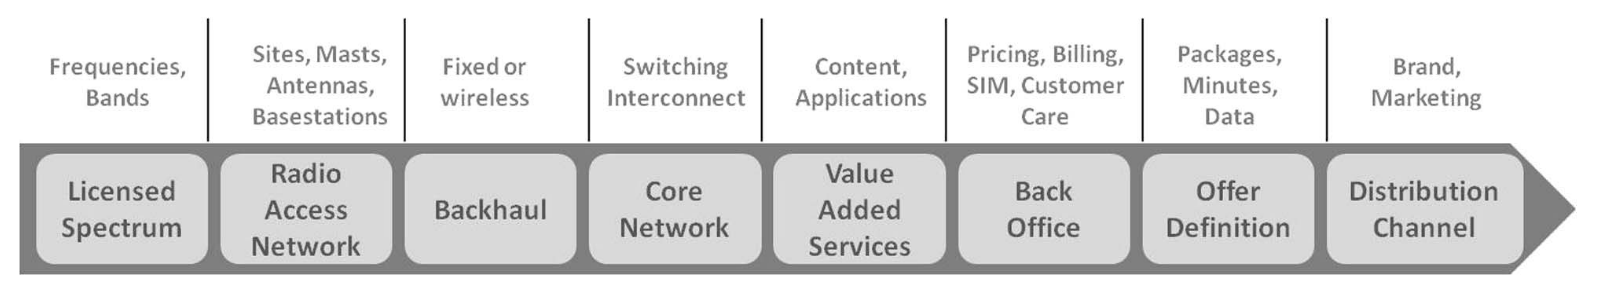
\includegraphics[width=\linewidth]{ClassicNetworkValueChain}
	\caption[Typical MNO value chain]{\small Typical MNO value chain~\cite{6737248}}
	\label{fig:ClassicNetworkValueChain}
\end{figure}

Specialization of networks and the entities involved in the network can improve the cost efficiency of the network.  According to Beckman and Smith~\cite{1421931}: ``Extensive vertical integration is a characteristic of an immature product.  As the product increases in complexity, it is no longer possible to [provide] an end-to-end solution.'' In both examples, the MVNO adds value to the traditional value chain by specializing in segments (e.g., marketing or service creation) that are different from the segments (e.g., network maintenance) still handled by the owner and operator of the network resources.

By focusing on the strengths provided by virtualization, more value can be generated through specialization.  Doyle et al.~\cite{6737248} investigates the value chain with this segmentation in mind and introduces the Networks without Borders (NwoB) approach as a new service-oriented network with a proposed new value chain (Fig. \ref{fig:NwoBValueChain}~\cite{6737248}).  The network under the NwoB approach is entirely service-oriented, where the network responds to services and connectivity is tailored for the service.  Services have a wider meaning than the voice, text, and data of a typical MNO.  Services also include that of Netflix-like or real-time video streaming, IoT applications, or various types of over-the-top services.  Each service would be provided by a service provider that compensates the virtual network operator operating a virtual network constructed specifically for the purpose of that service; the virtual network is the service.  Unlike an MVNO which manages resources provided to it by agreement, the virtual network operator manages slices of virtual resources from a pool of all resources as provided through resource aggregating services.

\begin{figure}
	\centering
	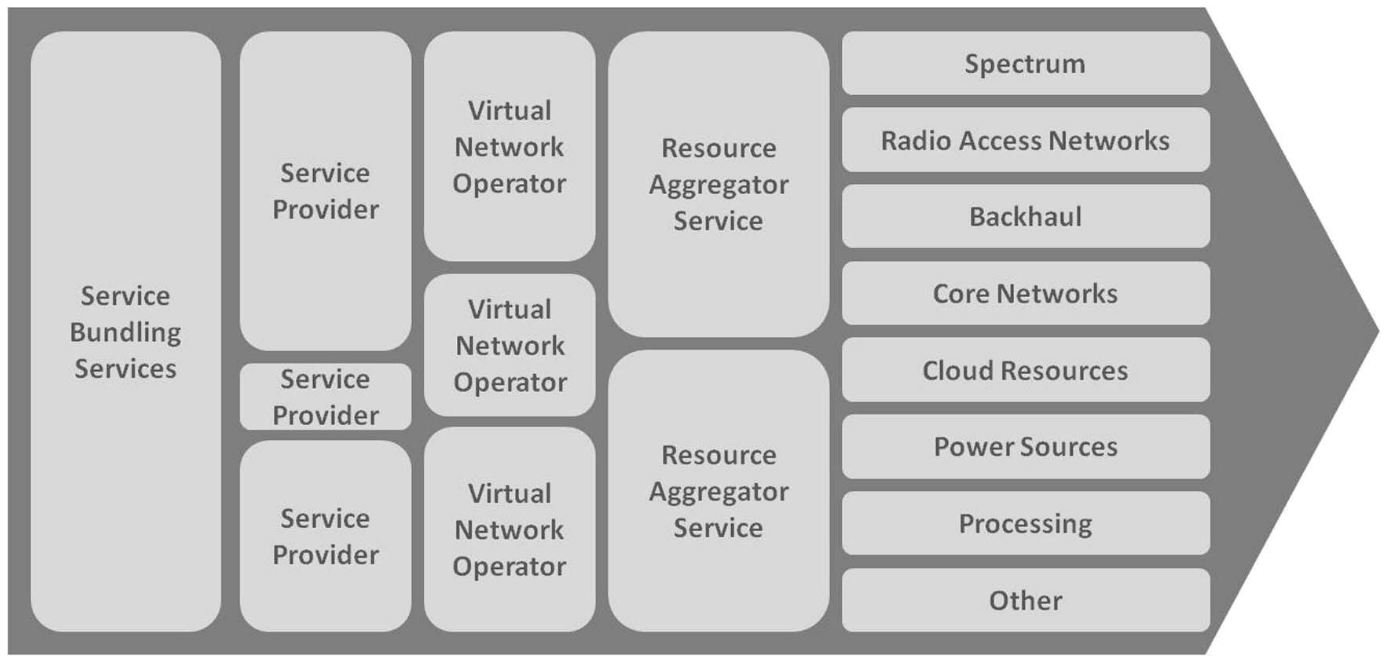
\includegraphics[width=\linewidth]{NwoBValueChain}
	\caption[Proposed network value chain under the NwoB paradigm]{\small Proposed network value chain under the NwoB paradigm~\cite{6737248}}
	\label{fig:NwoBValueChain}
\end{figure}

The benefits of this paradigm as proposed by Doyle et al.~\cite{6737248} are four-fold.  First, it provides specialization and independence for each stage, allowing service providers to focus on generating value from services provided.  Second, networks can be specialized for a service, reducing OpEx through extensive resource sharing.  Third, as resources are virtualized and pooled together, any resource (e.g., typical RAN, Wi-Fi, mmWave, raw spectrum) could be added with the pool and utilized for a network as its properties fit the network's needs.  Fourth, it lowers the barrier for entry and establishes services for new entities to fulfill.

\subsection{Virtualization Architecture in this Work} \label{subsec:virtualization_architecture}

Recognizing the critical nature of virtualization and resource allocation, this thesis develops and analyzes two methods for constructing virtualized wireless networks built on a virtualization architecture~\cite{MJ_CCNC_16, MJ_MECOMM_17} inspired by the NwoB paradigm presented by Doyle et al.~\cite{6737248}.  Fig. \ref{fig:VWNArchitecture}~\cite{MJ_CCNC_16, MJ_MECOMM_17} illustrates the three primary roles in this architecture: (1) the Resource Providers (RPs), (2) the Virtual Network Builders (VNBs), and (3) the Service Providers (SPs).

\begin{figure}
	\centering
	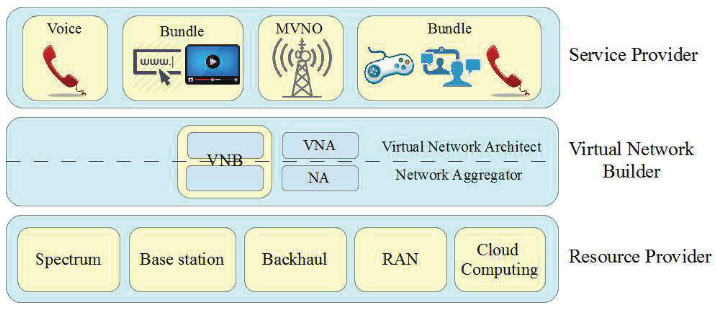
\includegraphics[width=\linewidth]{VWNArchitecture}
	\caption[VWN architecture as used in this work]{\small VWN architecture as used in this work~\cite{MJ_CCNC_16, MJ_MECOMM_17}}
	\label{fig:VWNArchitecture}
\end{figure}

RPs deploy and maintain the physical resources that are to be virtualized and offered for use within the virtualization framework and are the various entities that occupy the right-most column of segments (i.e., resources) in the NwoB value chain (Fig. \ref{fig:NwoBValueChain}~\cite{6737248}).  These resources can be in the form of any network-capable resource.  For example, the resources could be BSs as provided by a traditional MNO, a company- or individual-owned WLAN, femtocell access points, available licensed or unlicensed spectrum, or cloud computing.  An RP is then any entity that offers a virtualizable resource, such as a traditional MNO, company, or individual.  RPs maintain the resources, but also determine how the resource would be sliced and shared.

The VNB acts as resource aggregator, VWN constructor, and as intermediary between SPs and RPs.  Therefore, the VNB acts as a combination virtual network operator and resource aggregator in the NwoB value chain (Fig. \ref{fig:NwoBValueChain}~\cite{6737248}).  The VNB aggregates the resources maintained by individual RPs to establish the pool of available virtual resources.  The VNB also coordinates with SPs to understand the demands of their services and constructs VWNs tuned specifically to these demands.  By understanding the needs of the services provided by the SPs, the VNB will evaluate which virtual and virtualizable resources available from the RPs are needed to construct the optimal\footnote{In this network context, ``optimal'' is loosely defined to mean a network that provides the maximum demand satisfaction for the SP at the minimum cost to be paid to the RP.  These two requirements -- maximum demand satisfaction and minimum cost -- are frequently contradictory and need to be balanced by the VNB.} network for the SPs' needs, coordinate with the necessary RPs to obtain access to these resources for a given wholesale (OpEx) cost, and construct the network for the SPs to operate.  Multiple VNBs can coexist, each with their potentially overlapping set of RPs from which to aggregate resources.

SPs operate similarly to the service providers in the NwoB approach.  Primarily, an SP determines a service that they wish to provide, understands and enumerates the demands that are to be satisfied for that service, and provides the service over the VWN to their end users.  SPs can provide a wide range of services over the network.  The service could be a traditional MNO or be providing MNO-like services, such as voice calling and texting.  Services could cover specific applications, such as IoT, teleconferencing, augmented or virtual reality, or emergency services.  Other examples include traditional over-the-top services, such as Netflix-like or real-time (live) video streaming, social media (Facebook, Twitter, etc.), messaging (Skype, Groupme, etc.), or news/content feeds.  Further, an SP could also bundle several services, either through a single VWN built for the bundle, or by bundling services provided by several SPs.

Between these three entity roles, various interactions become possible.  The most common interactions are illustrated in Fig. \ref{fig:VWNArchitectureInteractions}~\cite{MJ_MECOMM_17}.  The interactions between the various entity roles are: (\emph{A}) among SPs; (\emph{B}) between the SPs and the VNBs; (\emph{C}) among VNBs; (\emph{D}) between the VNBs and the RPs; and (\emph{E}) among RPs.  It should be apparent that across each of these interactions is the imposition of costs as exchange for the transfer of services, networks, and resources.

\begin{figure}
	\centering
	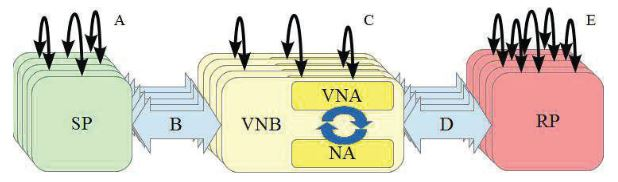
\includegraphics[width=\linewidth]{VWNArchitectureInteractions}
	\caption[Interactions between roles in the VWN architecture]{\small Interactions between roles in the VWN architecture~\cite{MJ_MECOMM_17}}
	\label{fig:VWNArchitectureInteractions}
\end{figure}

Interaction (\emph{A}) describes associations among various SPs.  This would typically occur in situations where a SP desires to bundle the services of several SPs, or when a SP wishes to utilize a specialized network operation from another SP.  Generally, this interaction would be performed manually over timescales of weeks or months.

Interaction (\emph{B}) describes associations directly between SPs and VNBs.  This would be one of the most common interactions within this framework.  This interaction is bidirectional.  In  the first direction, SPs would provide the VNB they are coordinating with the specific demands and needs for the service they are providing.  In the opposite direction, the VNB utilizes these conveyed needs and demands to construct a VWN and provide it for use to the service provider.  Ideally, this interaction is highly or entirely automated, with the interactions varying from minutes or hours to weeks or months based on the level of automation and the specifics of the interaction.  It will require optimization techniques and/or machine learning to achieve satisfactory results in this interaction.

Interaction (\emph{C}) describes associations among various VNBs.  Generally, such interactions may occur when a VNB does not have access to the appropriate virtual resources to satisfy interaction (\emph{B}) interactions.  Obvious examples include not having the necessary resources to provide adequate coverage over geographical areas or capacity in high-density environments.  These interactions would generally be performed manually over timescales of weeks or months.

Interaction (\emph{D}) describes associations between VNBs and RPs.  Similar to interaction (\emph{B}), this would be the other of the most common interactions within this framework.  It is also very important, as it establishes the mapping between the virtual and physical resources and builds the substrate that the framework is built upon.  VNBs interact with the RPs by making requests for new resources and releasing unneeded resources.  RPs interact with the VNBs by issuing updates, such as any changes to the resources in the VNBs' available pool of resources.  Updates such as these are potentially highly disruptive to the VNBs as the updates can impact a large number of VWNs managed by the VNBs.  With further similarity to interaction (\emph{B}), this interaction is highly dependent on automation; based on the level of automation, this interaction may occur over timescales of minutes or hours to weeks or months.

Interaction (\emph{E}) describes associations among various RPs.  In this interaction, various RPs establish connections with each other to facilitate proper mapping of physical resources to virtual through the use of quality of service (QoS) parameters that define the abstracted resources.  For example, a small-scale RP containing only an individual-owned femtocell could connect with a larger RP via this interaction so that the resource within the small-scale RP is visible for association with a VNB over interaction (\emph{D}) as handled by the larger RP.  These interactions could take seconds to weeks depending on the complexities of the RPs, their resources, and the amount of human involvement.

Other work has been completed using this architecture.  Abdel-Rahman et al.~\cite{MJ_CCNC_16} constructed several resource allocation models, including one-stage programs, two-stage programs, and a one-stage stochastic program, to investigate the efficacy of this virtualization architecture upon a preexisting set of resources.  The implementation focused on interaction (\emph{B}) from the perspective of the VNB, and showed that virtualization decreased the cost and idle capacity of the networks and increased demand satisfaction of the networks.

Cardoso et al.~\cite{MJ_MECOMM_17} expanded on this work by introducing a two-stage stochastic program to optimize interaction (\emph{B}).  The two-stage stochastic resource allocation similarly reduces cost and idle capacity of the VWN compared to the network without sharing.  However, no direct comparisons are made with the non-stochastic programs tested by Abdel-Rahman et al.~\cite{MJ_CCNC_16}.

Gomez et al.~\cite{pittir33631} utilized this architecture from an economics perspective.  Using a matching markets framework, they investigated the interaction of association between SPs and VNBs, such as the methods for how SPs indicate their needs and how VNBs indicate their VWN capabilities, and the fees that SPs will pay to partner for a VNB.  Gomez expanded on this work in her Ph.D. dissertation~\cite{pittir33130}.

The focus of this thesis is on optimization approaches largely in the context of interaction (\emph{B}).  This problem involves establishing how SPs convey the demands needed by the VNB to construct an optimal VWN for the service provided by the SP.  Further, the construction of the optimal VWN is sought within a short amount of time so that interaction (\emph{B}) can be completed over shorter timescales (e.g., minutes or hours) instead of longer (e.g., days, weeks, months).  With an optimal VWN in mind, construction of the VWN is inherently an optimization problem, and the search of expedient solutions lays within the study of optimization.

\section{Review of Optimization Methods} \label{sec:optreview}

In this thesis, I address the problem of the creation of optimal networks by a VNB that satisfy the specific demands of SPs using a pool of resources provided by a set of RPs.  This is naturally an optimization problem, in which some objective function is either minimized or maximized.  At it's most basic, optimization techniques (e.g., linear programming, integer programming) will find the set of input parameters that minimize or maximize a single decision variable -- the value of the objective function -- in context of a set of constraints.

\subsection{Stochastic Programming}	\label{subsec:optreview_stoch}

Standard linear and integer programming requires complete, certain knowledge of all parameters that affect the functions or model being optimized (i.e., the model's parameters and functions must be deterministic).  Communications, especially wireless communications, can be highly non-deterministic as the communication channel introduces a large amount of uncertainty.  Stochastic programming provides a powerful mathematical tool to handle optimization under such uncertainties.

Stochastic programming has been recently exploited to optimize resource allocation in various types of wireless communications operating under uncertainties.  Abdel-Rahman et al.~\cite{MJ_CCNC_16} exploit stochastic optimization within the framework of the virtualization architecture presented in \Cref{subsec:virtualization_architecture} to minimize the cost of resource allocation by introducing probabalistic QoS guarantees.  Cardoso et al.~\cite{MJ_MECOMM_17} expand on that work by introducing a second stage to balance maximizing demand satisfaction while minimizing cost.  Further examples include resource allocation in dynamic spectrum access (DSA) networks~\cite{MJ_TW_13}, optimal orchestration of LTE-U networks utilizing Wi-Fi access points~\cite{MJ_WCNC_16}, resource allocation in opportunistic LTE-A networks considering end user rate demand satisfaction~\cite{MJ_DySPAN_15}, resource allocation for OFDMA-based cognitive radios considering primary user system interference~\cite{CC_OFDMA}, and predictive resource allocation for energy-efficient video streaming to mobile end users~\cite{CC_video}.

Introducing stochastic parameters and constraints allows the optimization model to consider probabilities within the optimization.  In the case of resource allocation in networks, it may be possible to allocate enough resources to satisfy all end-user demand.  Such an optimization may require too many resources to be economical considering the law of diminishing returns, with the solution being cost prohibitive.  It is much cheaper to solve such that 95\% or 99\% of demand is satisfied, leaving some demand unsatisfied.

However, standard linear programming techniques cannot solve models with stochastic parameters.  Stochastic programming therefore requires converting the stochastic program into its deterministic equivalent program (DEP) which replaces all stochastic variables with deterministic variables~\cite{stochprogramming}.  The process of forming a DEP from a stochastic program involves converting each stochastic variable into a set of all possible scenarios and scenario probabilities.  These scenarios and scenario probabilities are present within the model as a new dimension and weight for the now-deterministic variable.  To fully encapsulate the stochastic variable, the deterministic equivalent variable may be composed of an infinite set.

Resource allocation problems are typically some form of integer programming--in which all decision variables (unknowns) are integers--or mixed integer programming--in which some decision variables (unknowns) are integers.  Both integer and mixed integer programs are generally\footnote{Some subclasses of integer and mixed integer programs are efficiently solvable, but these are the exception.  Several classic NP-Complete (a subset of NP-Hard) problems~\cite{Karp1972} are integer programs and mixed integer programs.} considered NP-hard\footnote{Finding the minimum resource allocation that provides coverage over a geographic area falls within a category of problems referred to as \emph{minimum set cover problems}.  It is apparent that the problem considered in this thesis--specifically the stochastic program proposed in \Cref{sec:stochopt}--is some form of minimum set cover problem; specifically, it might be referred to as a capacitated set cover problem.  Minimum set cover problems are provably NP-hard and typically rely on approximation solutions to solve in a feasible amount of time~\cite{Korte:2007:CombOptimization}.}.  As the programs increase in scope, they become more computationally complex to solve; accounting for the scenarios of the previously stochastic variables further increases this complexity.  Finding the optimal solution may require more time than is feasible; in the worst case, these problems run in exponential time complexity.

\subsection{Metaheuristic Approaches} \label{subsec:optreview_meta}

The use of heuristic or metaheuristic algorithms can provide close-to-optimal solutions in much better time.  Examples include hill climbing, simulated annealing, ant colony optimization, and particle swarm optimization.  Each of these approaches are iterative techniques.

Hill climbing starts with an arbitrary solution and makes incremental changes to variables, finding a new solution.  If the new solution is better than the previous, the new solution is iterated upon.  This continues until no further improvements can be made.  Hill climbing will only find the local maximum close to the initial arbitrary solution, and is best in convex problems where the only local maximum is guaranteed to be the global maximum.

Simulated annealing is inspired by the process of annealing found in metallurgy, where metal is heated to the point where atoms can migrate, reducing defects in the crystalline structure.  In simulated annealing, the model has some notion of temperature, which represents the internal energy of the system, and states, which represent possible solutions to the system being optimized.  The system has an initial state, each state has an associated energy, and the system is attempting to reach the state of lowest energy.  On each iteration, the heuristic considers a neighboring state, and chooses to transition to the new state with a probability dependent on the energy of the current state, the energy of the neighboring state, and the temperature.  This transition can lead from a lower energy state (better) to a higher energy state (worse), and will do so more often while it has a higher temperature.  Gradually, the system will cool and decrease the temperature, which causes the system to tend to select states with lower energy; as the temperature drops, the systems overall energy drops.  When the temperature reaches zero, the system will only transition to states of lower energy (i.e., that are more optimal), reducing to the hill climbing algorithm.

Ant colony optimization is inspired by the behavior of ants.  A colony of ants move around independently trying to find food, laying pheromones on the taken path.  Upon crossing paths, ants have a probabilistic chance to follow the new path based on the strength of the pheromones of the new and old paths.  Over time, pheromones evaporate, and paths less taken will weaken.  Longer paths, since they take longer to traverse and will be reinforced less often, will also weaken.  This has benefits over approaches like simulated annealing because it adapts in real time.

In particle swarm optimization, a number of candidate solutions, called particles, are created that move semi-chaotically.  In each iteration, every particle will move according to its velocity.  Each particle has it's best known position, and it's velocity updates in a way that is guided by their own best known position and the swarm's best known position.  This allows a large portion of the search space to be investigated, with candidate solutions exploring regions containing local maxima until it settles to exploit and find the best found local maxima.

In this thesis, I utilize a genetic algorithm as an approach for optimization.  A genetic algorithm is a form of evolutionary algorithm, a set of algorithms which are inspired by biological evolution and natural selection.  Each iteration is called a \emph{generation} and is composed of a number of candidate solutions called \emph{individuals}.  Each individual is defined by a \emph{chromosome} which details the specific candidate solution.  During each generation, every individual is evaluated on its \emph{fitness}, a function dependent on the individual's chromosome; the higher the individual's fitness, the more optimal the individual.  Individuals called \emph{parents} are then randomly selected to pass their chromosome onto the next generation in a process called \emph{selection}; in selection, more fit individuals are more likely to be selected.  With a certain probability, groups of parents will undergo \emph{crossover} and exchange the data contained within their chromosomes to form new \emph{children} that are a mixture of the parents; if mixing does not occur, the parents are cloned into the next generation as children.  Then, individual bits within the children's chromosomes have a chance to flip, or \emph{mutate}.  The resulting children from crossover and mutation form the entire next generation.

Since chromosomes from fitter individuals are more likely to pass on to subsequent generations, generations gradually become fitter.  Through crossover, fit chromosomes may combine to form fitter children that proliferate; less fit children are often also formed, but are generally not selected for later generations.  Mutation introduces diversity into the generations, which expand the exploration of the search space.  More details, including that of implementation and variants, will be expanded upon in \Cref{sec:ga}.

Genetic algorithms have been used previously as approaches for simplifying the search spaces of large, complex stochastic optimization problems.  For example, Cui et al.~\cite{7257198} used a genetic algorithm where each chromosome defined a subproblem of larger resource allocation optimization problem, and the fitness was evaluated by solving the subproblems with linear programming optimization methods.  One approach investigated in this thesis coordinates a genetic algorithm with an optimization program wherein the genetic algorithm solves for and fixes a decision variable to simplify the larger optimization program.  Hybrid approaches (e.g., Cui et al.) and other effective metaheuristic algorithms (e.g., ant colony optimization, particle swarm optimization, neural networks, and machine learning) are worth investigating in the context of the posed VWN architecture, but beyond the scope of this thesis.

\section{Thesis Objective} \label{sec:objective}

The objective of this thesis is to develop two approaches to joint resource allocation to construct a set of a VWNs and adaptively slice the selected resources to allocate to the individual VWNs.  A model will be presented as the context for these approaches, expanding upon the VWN architecture proposed in \Cref{subsec:virtualization_architecture}.  The validity of this model will be restricted to the scope of cellular networks using generic base stations as its resources.  The two proposed approaches will be performed within the VNB, and evaluated in four cases that differ in the resources provided by the RPs and service demands to be satisfied by the SPs.  Accordingly, the efficacy of these approaches will be measured primarily by the optimality of the solutions, such as cost and network service demand satisfaction, and the run time, providing the VNB with a sufficient solution in a reasonable amount of time.

\section{Thesis Outline} \label{sec:outline}

This thesis is organized as follows.  \Cref{ch:vnbmodel} defines the model used for the resource allocation methods explored in this thesis.  Further, \Cref{ch:vnbmodel} also details the two-stage stochastic optimization problem which optimally performs resource selection and slicing as a basis of approaches presented within this work.  \Cref{ch:approaches} establishes the two approaches investigated to provide solutions to the optimization problem posed in \Cref{ch:vnbmodel}: a sampled deterministic equivalent program which solves the problem as a whole and a genetic algorithm that simplifies the problem by providing an estimated optimal resource selection.  \Cref{ch:sim} tests these two approaches by presenting four data sets that mimic real world cellular networks and evaluates the results.  \Cref{ch:conc} contains the conclusions and proposed future work in this area.
\fi

\iftrue
\pagebreak
\chapter{Virtual Network Builder Model} \label{ch:vnbmodel}

This chapter establishes the mathematical foundation for this thesis.  First, a geographic model is presented defining an area of interest, the pool of resources maintained by the RPs for use by the VNB, and a characterization of the service demand of each SP.  Second, a specific demand model, based on the empirical analysis of collected cellular network traces, is presented.  This is the demand model that will be used throughout this thesis.  Third, a two-stage stochastic program is developed to model the problem of resource selection and adaptive slicing within the VNB.

Throughout this thesis, stochastic variables will be differentiated from deterministic variables with a tilde ($\sim$) placed above the symbol.

\section{Network Area Definitions} \label{sec:networkdefs}

Consider a geographic region, $\mathcal{R}$, of width $X$ meters and length $Y$ meters that contains a VNB and a set $\mathcal{S} \defeq \left\{ 1,\, 2,\, \ldots,\, S \right\}$ of virtualized resources (i.e., BSs) the VNB has aggregated for use in the construction of VWNs.  The pool of BSs, $\mathcal{S}$, is mapped to physical BSs owned and maintained by RPs and made available for use through contracts between the RPs and the VNB.  The contract-negotiated cost for the VNB to lease BS $s \in \mathcal{S}$ is denoted by $c_s$.  The costs for the BSs used within a constructed VWN are passed to the SPs as part of the overall cost of the network.  The rate capacity of BS $s \in \mathcal{S}$ is denoted by $r_s$ and its coverage radius is denoted by $b_s$.

Let $\mathcal{N} \defeq \left\{ 1,\, 2,\, \ldots,\, N \right\}$ be the set of SPs seeking a VWN with coverage within the region $\mathcal{R}$.  An SP $n \in \mathcal{N}$ associates with the VNB to create the desired VWN.  Through this association, SP $n$ must coordinate with the VNB to indicate the demands of the intended service the VWN would need to satisfy.  SP $n$ must know and communicate to the VNB the estimated geographic distribution of the service's traffic demand density (or demand \emph{intensity}) as a function, $\lambda_n\left( x,\, y \right),\, n \in \mathcal{N},\, x \in \left[ 0,\, X \right],\, y \in \left[ 0,\, Y \right],\,$ in terms of $\frac{\text{bits}}{\text{km}^2}$.  The demand intensity function could be in the form of a continuous function or as discrete pixels (e.g., a bitmap), and indicates the locations of necessary coverage and the desired capacity within specific regions of the area.  Examples of possible maps could be for services such as localized video streaming (specific, localized coverage with high regional capacities) or MNO-like voice lines (broad coverage with comparatively low capacity).  For an example of $\lambda_n$, see \Cref{subsec:networkdefs_sslt}.

Further, the SP would also provide the desired or needed percent demand satisfaction rate\footnote{Percent demand satisfaction rate refers to the percent of the demand described by $\lambda_n$ that is satisfied by VWN constructed by the VNB.  In this context, it is the percent of total requested demand that is sliced resources by the VNB.  This will be more formally described later in \Cref{sec:stochopt} (\cref{eq:VWN_demand_sat}) and evaluated during simulations in \Cref{ch:sim}.} for the service.  Some services, such as those related to emergency services, must have nearly 100\% demand satisfaction.  Others, such as generic voice lines or video streaming, may be able to tolerate some unsatisfied demand as a tradeoff for decreased network leasing or operational costs.

$\lambda_n$ describes the geographic distribution of SP $n \in \mathcal{N}$ within $\mathcal{R}$.  At any instantaneous point in time, $\lambda_n$ is realized as a set of discrete demand points (each representing e.g., user equipment).  Let $\mathcal{M}_n \defeq \left\{1,\, 2,\, \ldots,\, M_n\right\}$ be this set of demand points SP $n$ is attempting to satisfy with its service at a given point in time.  Each demand point $m \in \mathcal{M}_n$ is seeking to connect to the VWN operated by SP $n \in \mathcal{N}$ and is located within the domain of $\mathcal{R}$ (i.e., $\left( \tilde{x}_{m_n},\, \tilde{y}_{m_n} \right),\, \tilde{x}_{m_n} \in \left[ 0,\, X \right],\, \tilde{y}_{m_n} \in \left[ 0,\, Y \right]$).  Demand point locations are stochastically determined by the distribution of traffic as described by the demand intensity function $\lambda_n$.  A realization of these demand points can be found as a two-dimensional non-stationary (or inhomogeneous) Poisson point process (PPP) using $\lambda_n$ as it's spatial intensity function.

For purposes of visualization or compuation, this non-stationary PPP is generatable using an accept-reject method~\cite{leeds:nsPPPgeneration}.  A stationary PPP is generated relative to the maximum value of the traffic demand density function within $\mathcal{R}$.  That is, a number of points generated within the region is selected from a Poisson random variable with parameter (or mean) $\lambda_{n,\max}*X*Y$, where $\lambda_{n,\max}$ is the maximum value of $\lambda_n$ within $\mathcal{R}$.  Each point is then independently and uniformly distributed (i.e., each point has a location $\left( x,\, y \right)$ with $x \sim \mathcal{U}\left( 0,\, X \right)$\footnote{$\mathcal{U}\left( a,\, b \right)$ refers to a random variable uniformly distributed over the domain $\left[ a,\, b \right]$, where $a < b$.} and $y \sim \mathcal{U}\left( 0,\, Y \right)$) over $\mathcal{R}$.  Then, each point undergoes the accept-reject procedure to inhomogenize the stationary PPP.  Each point is kept with a probability of the ratio of the value of the intensity function at that point's location to the maximum value of the intensity function.  That is, for each point in the PPP a uniform random variable, $P \sim \mathcal{U}\left( 0,\, 1 \right)$, is generated and the point is either \emph{accepted} and kept or \emph{rejected} and discarded according to

\ifisdoublespacing
\begin{singlespacing}
\begin{equation} \label{eq:nsPPPaccrej}
\begin{cases}
	\text{the $i^{\text{th}}$ point is kept},& \text{if } P \leq \frac{\lambda\left( x_i,\, y_i \right)}{\lambda_{n,\max}};\\
	\\
	\text{the $i^{\text{th}}$ point is discarded},& \text{otherwise,}
\end{cases}
\end{equation}
\end{singlespacing}
\else
\begin{equation} \label{eq:nsPPPaccrej}
\begin{cases}
	\text{the $i^{\text{th}}$ point is kept},& \text{if } P \leq \frac{\lambda\left( x_i,\, y_i \right)}{\lambda_{n,\max}};\\
	\text{the $i^{\text{th}}$ point is discarded},& \text{otherwise,}
\end{cases}
\end{equation}
\fi

\noindent where $x_i$ and $y_i$ are the x- and y-coordinates of the $i^{\text{th}}$ point of the stationary PPP.

Each demand point $m \in \mathcal{M}_n$ loads the VWN of SP $n \in \mathcal{N}$ with point traffic demand denoted by $d_{n}$.  So that the total demand described by $\lambda_n$ is allocated by the points in $\mathcal{M}_n$, the overall demand 

\begin{equation} \label{eq:demandintegral}
D_n = \int_0^X \int_0^Y \lambda_n\left( x,\, y \right) dy \, dx, n \in \mathcal{N},
\end{equation}

\noindent of the demand density distribution is evenly distributed such that

\begin{equation} \label{eq:pointdemand}
d_{n} = \frac{D_n}{M_n},\, n \in \mathcal{N}.
\end{equation}

Let $\tilde{u}_{mns} \in \left[ 0,\, 1 \right]$ represent the normalized capacity (with respect to $r_s$) of BS $s \in \mathcal{S}$ at point $m \in \mathcal{M}_n, n \in \mathcal{N},$ associated with SP $n \in \mathcal{N}$ (i.e., the normalized maximum rate that a user can receive at point $m$ from BS $s$).  Specifically,

\ifisdoublespacing
\begin{singlespacing}
\begin{equation} \label{eq:umns}
\tilde{u}_{mns} \defeq
	\begin{cases}
		0,& \text{if demand point $m$ of SP $n$ is located more than $b_s$ meters from}\\
		& \text{\tab from BS $s$;}\\
		\\
		1,& \text{if demand point $m$ of SP $n$ is located within a small distance of}\\
		& \text{\tab BS $s$;}\\
		\\
		(0,\, 1),& \text{otherwise.}
	\end{cases}
\end{equation}
\end{singlespacing}
\else
\begin{equation} \label{eq:umns}
\tilde{u}_{mns} \defeq
	\begin{cases}
		0,& \text{if demand point $m$ of SP $n$ is located more than $b_s$ meters from}\\
		& \text{\tab from BS $s$,}\\
		1,& \text{if demand point $m$ of SP $n$ is located within a small distance of}\\
		& \text{\tab BS $s$}\\
		(0,\, 1),& \text{otherwise.}
	\end{cases}
\end{equation}
\fi

It is apparent that $\tilde{u}_{mns}$ will vary according to the path-loss characteristics of the environment, the locations of the demand points, and other various factors.  In some instances, it can be beneficial to simplify this definition such that

\ifisdoublespacing
\begin{singlespacing}
\begin{equation} \label{eq:umns_simp}
\tilde{u}_{mns} \defeq
	\begin{cases}
		0,& \text{if demand point $m$ of SP $n$ is located more than $b_s$ meters from}\\
		& \text{\tab BS $s$;}\\
		\\
		1,& \text{otherwise (i.e., if demand point $m$ of SP $n$ is located less than}\\
		& \text{\tab or equal to $b_s$ meters from BS $s$).}\\
	\end{cases}
\end{equation}
\end{singlespacing}
\else
\begin{equation} \label{eq:umns_simp}
\tilde{u}_{mns} \defeq
	\begin{cases}
		0,& \text{if demand point $m$ of SP $n$ is located more than $b_s$ meters from}\\
		& \text{\tab BS $s$;}\\
		1,& \text{otherwise (i.e., if demand point $m$ of SP $n$ is located less than}\\
		& \text{\tab or equal to $b_s$ meters from BS $s$).}\\
	\end{cases}
\end{equation}
\fi

\noindent Under this definition, $\tilde{u}_{mns}$ is binary and wholly determined by the stochastic locations of the demand points and the fixed locations and ranges of the BSs.

From the perspective of the VNB, each SP is only distinguishable by its overall demand characteristics.  These demand characteristics are defined by the SPs' demand density distributions.  The VNB must construct a VWN for each SP, but for optimal VWNs to be created, the VNB must consider the demands of all SPs simultaneously and in context of each other.  For the VNB, all SP demand points are indistinguishable and independent.  Therefore, the VNB considers a single set of demand points

\begin{equation} \label{eq:union_M}
\mathcal{M} \defeq \bigcup_{n \in \mathcal{N}} \mathcal{M}_n = \left\{ 1,\, 2,\, \ldots,\, M \right\},
\end{equation}

\noindent where $M = \sum_{n \in \mathcal{N}} M_n$, with demands $d$ and stochastic normalized capacities $\tilde{u}_{ms},\, m \in \mathcal{M},\, s \in \mathcal{S}$.  $\mathcal{M}$ can be considered a set of demand points associated with a superposition of PPPs with intensity $\lambda = \sum_{n \in \mathcal{N}} \lambda_n$.

\subsection{Example Demand Distribution; The SSLT Model} \label{subsec:networkdefs_sslt}

One major assumption made in \Cref{sec:networkdefs} is that SPs must communicate the demand characteristics (i.e., $\lambda_n$) of their service to the VNB to properly facilitate VWN construction.  In this subsection, I establish an example model demonstrating the demand characteristics to be communicated by generating an example hypothetical demand intensity function.  For testing the approaches for VWN construction presented in \Cref{ch:approaches}, this example is the fundamental model used for simulating SP demand in cellular network-based services.

Gotzner et al.~\cite{686105} have shown that a log-normal distribution\footnote{It has also been shown that traffic distributions in cellular networks can be approximated by a Weibull distribution~\cite{6757900}, by mixtures of log-normal distributions~\cite{5936263, 6757900}, or by an $\alpha$-stable distribution~\cite{7202841}.} can approximate traffic demand in real-world cellular networks.  It has also been shown that traffic distributions are spatially correlated~\cite{5936263, eigenplaces}.  Lee et al.~\cite{6554749, 6757900} presented the Scalable, Spatially-correlated, and Log-normally distributed Traffic (SSLT) model to emulate the characteristics of real world cellular data networks.  This model is flexible and can be adjusted to simulate numerous cellular networks, and can characterize the demand of a supposed SP in a way that mimics real-world data.  I use a variant of the SSLT demand model presented by Lee et al., which I altered to be a continuous function serving as a continuous or pixelated demand density map.

To generate this spatial SSLT model distribution over the area of consideration, an initial Gaussian field, $\lambda^G = \lambda^G\left( x,\, y \right),\, x \in \left[ 0,\, X \right],\, y \in \left[ 0,\, Y \right]$, is generated by
\begin{equation} \label{eq:lambdaG}
\lambda^G\left( x,\, y \right) = \frac{1}{L} \; \sum_{l=1}^L \cos\left( i_l x + \phi_l \right) \; \cos\left( j_l y + \psi_l \right)
\end{equation}
where $\mathcal{L} \defeq \left\{ 1,\, 2,\, \ldots,\, L \right\}$ is a set of the products of two cosines with stochastic angular frequencies $i_l,\, j_l\, \sim \mathcal{U}\left( 0,\, \omega_{\max} \right),\, l \in \mathcal{L}$ and phases $\phi_l,\, \psi_l\, \sim \mathcal{U}\left( 0,\, 2 \pi \right),\, l \in \mathcal{L}$.  As $L$ increases, it is expected that $\lambda^G$ approaches a Gaussian random field according to the central limit theorem.

According to Lee et al.~\cite{6554749}, $\lambda^G$ is spatially correlated with autocorrelation function
\begin{equation} \label{eq:sslt_autocorrelation}
R\left( dx,\, dy \right) = \mathbb{E}\left[ \lambda^G\left( x,\, y \right) \; \lambda^G\left( x + dx,\, y + dy \right) \right] = \frac{1}{4L} \; \sinc\left( \omega_{\max} dx \right) \; \sinc\left( \omega_{\max} dy \right).
\end{equation}
The autocorrelation function is notably dependent on the maximum angular frequency defining $\rho^G$, $\omega_{\max}$.  As $\omega_{\max}$ increases, the demand of adjacent regions become less correlated.  $\omega_{\max}$ is effectively a measure of the inhomogeneity of $\rho^G$.  This effect of $\omega_{\max}$ on the inhomogeneity of $\lambda^G$ is shown in Fig. \ref{fig:lambdaG}; Fig. \ref{fig:lambdaG_4pi-300} fluctuates more rapidly than Fig. \ref{fig:lambdaG_2pi-300}, which is generated from a smaller $\omega_{\max}$.

\begin{figure}[!ht]
\centering
\begin{subfigure}{.45\textwidth}
	\centering
	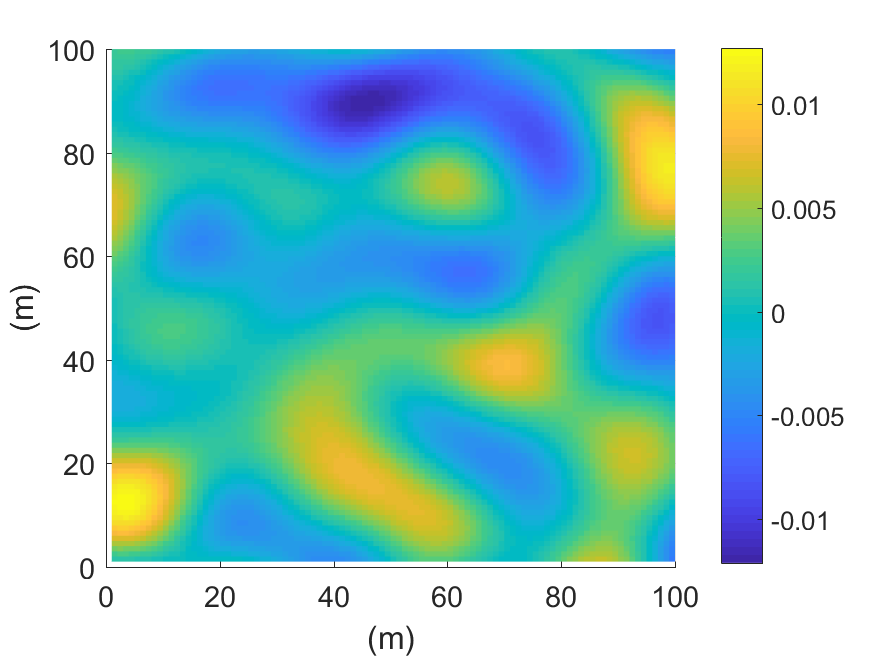
\includegraphics[width=1\linewidth]{lambdaG_O2pi-300_L100000_X100_Y100}
	\caption{\small $\omega_{\max}=\frac{2 \pi}{30}$}
	\label{fig:lambdaG_2pi-300}
\end{subfigure}
\hspace{0.5cm}
\begin{subfigure}{.45\textwidth}
	\centering
	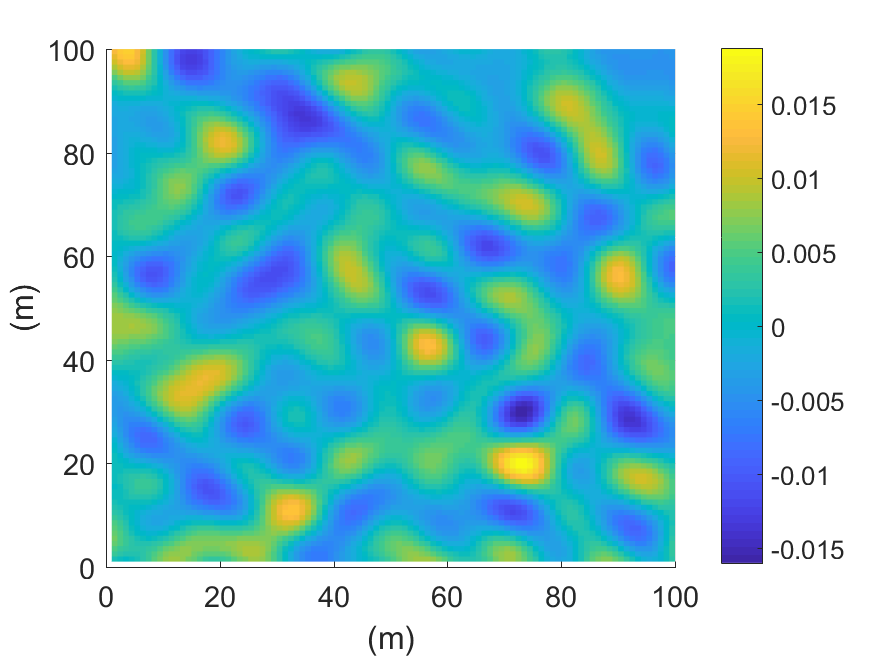
\includegraphics[width=1\linewidth]{lambdaG_O4pi-300_L100000_X100_Y100}
	\caption{\small $\omega_{\max}=\frac{4 \pi}{30}$}
	\label{fig:lambdaG_4pi-300}
\end{subfigure}
\caption[Example Gaussian random fields for SSLT demand model generation]{\small Two example Gaussian random fields (i.e., $\lambda^G$) for generating the SSLT demand model, varying by $\omega_{\max}$.  $L = 100000,\, X = 100,\, Y = 100$}
\label{fig:lambdaG}
\end{figure}

The approximate Gaussian distribution $\lambda^G$ is then normalized to a standard normal distribution\footnote{A standard normal distribution is a Gaussian distribution with mean $\mu = 0$ and variance $\sigma = 1$.}, $\lambda^S = \lambda^S\left( x,\, y \right),\, x \in \left[ 0,\, X \right],\, y \in \left[ 0,\, Y \right]$,

\begin{equation} \label{eq:lambdaS}
\lambda^S\left( x,\, y \right) = \frac{\lambda^G\left( x,\, y \right) - \mean{\lambda^G}}{\sqrt{\var\left( \lambda^G \right)}},
\end{equation}

\noindent where $\var\left( \lambda^G \right) = \mathbb{E}\left[ \left( \lambda^G \right)^2 \right] - \mathbb{E}\left[ \lambda^G \right]^2$ is the variance of $\lambda^G$ and $\mean{\lambda^G} = \mathbb{E}\left[ \lambda^G \right]$ is the mean of $\lambda^G$.  While this could be mathematically derived, in practice $\var\left( \lambda^G \right)$ and $\mean{\lambda^G}$ are the sample variance and mean which are empirically found from a set of uniformly distributed sampled points (i.e., a simple random sample of $\lambda^G$).

The final log-normal distribution, $\lambda = \lambda\left( x,\, y \right), x \in \left[ 0,\, X \right], y \in \left[ 0,\, Y \right]$, is determined by assigning location ($\mu$) and scale ($\sigma$) parameters to $\lambda^S$ according to
\begin{equation}\label{eq:lambdaLN}
\lambda\left( x,\, y \right) = \exp\left( \sigma \; \lambda^S\left( x,\, y \right) + \mu \right).
\end{equation}

Fig. \ref{fig:lambda} shows the resulting SSLT demand density distribution, $\lambda$, generated from the $\lambda^G$ fields displayed in Fig. \ref{fig:lambdaG} with default location and scale parameters (i.e., $\mu = 0,\, \sigma = 1$).  By controlling the maximum angular frequency of the originating Gaussian random field, $\omega_{\max}$, and the log-normal location and scale parameters, the SSLT model can be used to simulate the demand characterization of a hypothetical SP service.

\begin{figure}[!ht]
\centering
\begin{subfigure}{.45\textwidth}
	\centering
	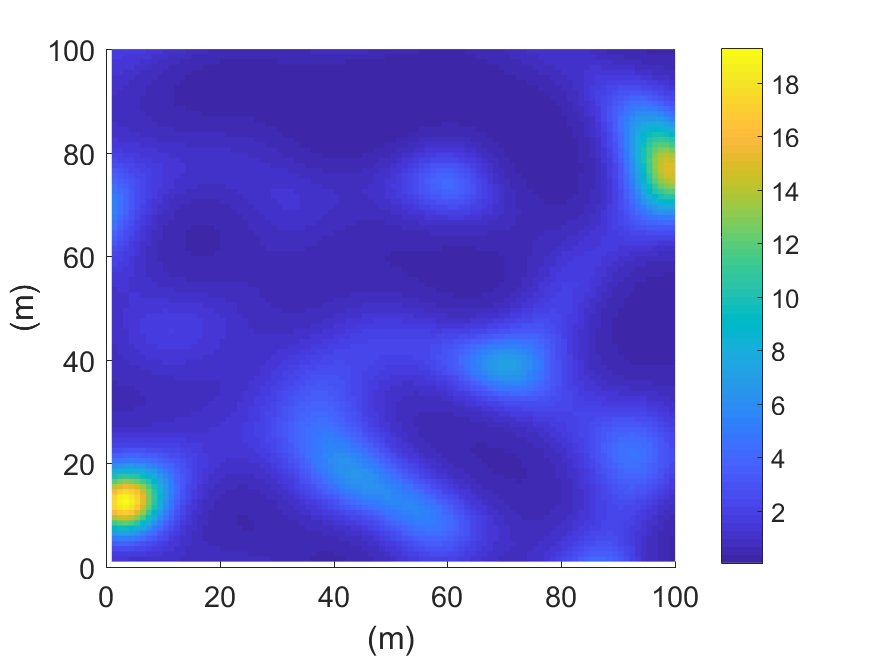
\includegraphics[width=1\linewidth]{lambda_O2pi-300_L100000_X100_Y100}
	\caption{\small $\omega_{\max}=\frac{2 \pi}{30}$}
	\label{fig:lambda_2pi-300}
\end{subfigure}
\hspace{0.5cm}
\begin{subfigure}{.45\textwidth}
	\centering
	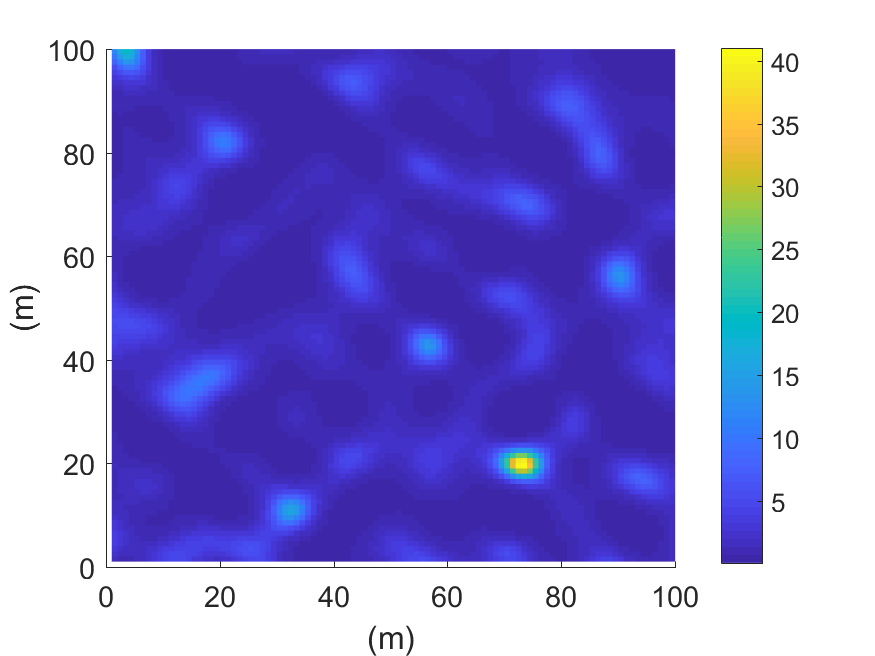
\includegraphics[width=1\linewidth]{lambda_O4pi-300_L100000_X100_Y100}
	\caption{\small $\omega_{\max}=\frac{4 \pi}{30}$}
	\label{fig:lambda_4pi-300}
\end{subfigure}
\caption[Generated example SSLT demand fields]{\small Two SSLT demand fields generated from the $\lambda^G$ demand fields displayed in Fig. \ref{fig:lambdaG}. $\mu = 0,\, \sigma = 1$}
\label{fig:lambda}
\end{figure}

Lee et al.~\cite{6554749, 6757900} implement their proposed SSLT demand model as a discrete pixelated set of rectangular cells, the value of which indicates the overall demand located within that cell's region.  Each demand point located within the SSLT area has an identical amount of demand associated with it.  The value of each cell represents the number of homogeneous demand points located within that cell, and these demand points are uniformly distributed within that cell.

I deviate from their implementation by leaving the SSLT distribution as a continuous function representing the overall demand of the region, and only pixelate it for visualization purposes.  To generate discrete demand points, I generate a non-stationary PPP using $\lambda$ as the spatial intensity function as described by the accept-reject method (\cref{eq:nsPPPaccrej}) described previously.  This allows the specific number of demand points to be controlled and accommodates for the assumption that the SSLT demand model is an overall distribution of demand points rather than each cell operating as independent PPP.  Fig. \ref{fig:lambda_nsPPP} shows a realization of demand points distributed as a non-stationary PPP.

\begin{figure}[!ht]
\centering
\begin{subfigure}{.45\textwidth}
	\centering
	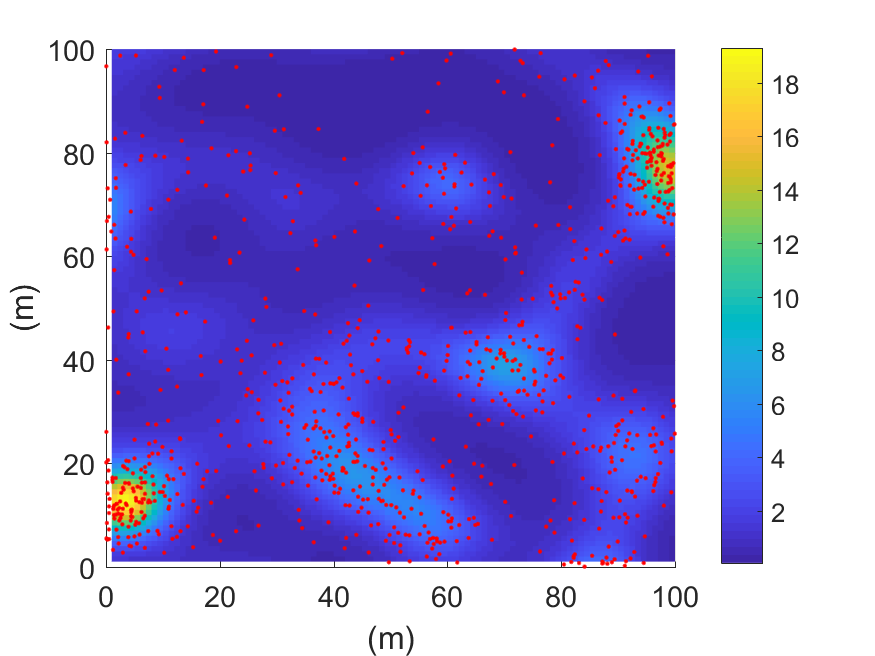
\includegraphics[width=1\linewidth]{lambda_nsPPP-400_O2pi-300_L100000_X100_Y100}
	\caption{\small $\omega_{\max}=\frac{2 \pi}{30}$}
	\label{fig:lambda_nsPPP_2pi-300}
\end{subfigure}
\hspace{0.5cm}
\begin{subfigure}{.45\textwidth}
	\centering
	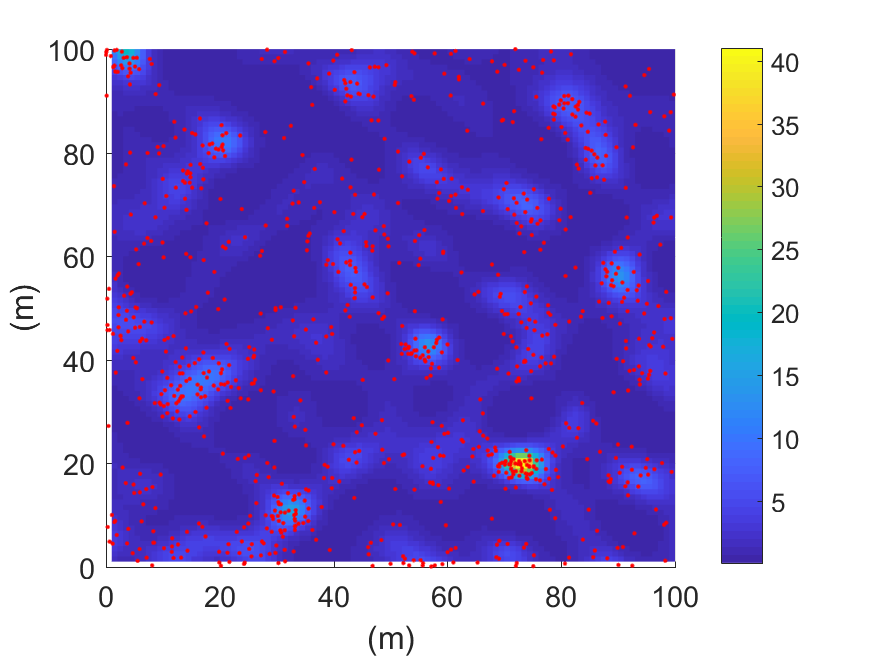
\includegraphics[width=1\linewidth]{lambda_nsPPP-400_O4pi-300_L100000_X100_Y100}
	\caption{\small $\omega_{\max}=\frac{4 \pi}{30}$}
	\label{fig:lambda_nsPPP_4pi-300}
\end{subfigure}
\caption[Realizations of example SSLT demand point distributions]{\small Example demand point realizations distributed according to the described non-stationary PPP with 400 demand points.}
\label{fig:lambda_nsPPP}
\end{figure}

This SSLT model is used in \Cref{ch:sim} to generate SP service demand and end-user demand points while testing the approaches described in \Cref{ch:approaches}.

\section{Stochastic Optimization} \label{sec:stochopt}

As presented in \Cref{sec:networkdefs}, the VNB present within the $\mathcal{R}$ must construct a set of VWNs to satisfy the needs of the services the various SPs seek to provide.  Each service provider provides a characterization of its demand, such as the SSLT model presented in \Cref{subsec:networkdefs_sslt}.  With this information, the VNB must select the subset of virtual resources available in $\mathcal{S}$ that minimizes the cost to the VNB, and associate slices of these resources to VWNs that optimally satisfy the SPs' demand.

I formulate the presented problem of resource selection as a two-stage stochastic optimization program (\cref{eq:SOPS1O,eq:SOPS1C1,eq:SOPS2O,eq:SOPS2C1,eq:SOPS2C2,eq:SOPS2C3,eq:SOPS2C4}).  Let $z_s,\, s \in \mathcal{S}$, be a binary decision variable defined as

\ifisdoublespacing
\begin{singlespacing}
\begin{equation} \label{eq:z_s}
z_s \defeq
	\begin{cases}
		1,& \text{if resource $s$ is selected to be sliced into a VWN;}\\
		\\
		0,& \text{otherwise.}
	\end{cases}
\end{equation}
\end{singlespacing}
\else
\begin{equation} \label{eq:z_s}
z_s \defeq
	\begin{cases}
		1,& \text{if resource $s$ is selected to be sliced into a VWN;}\\
		0,& \text{otherwise,}
	\end{cases}
\end{equation}
\fi

\noindent which establishes VNB resource selection.  Further let $\delta_{ms} \in \left[ 0 ,\, r_s \right],\, m \in \mathcal{M},\, s \in \mathcal{S}$, be a decision variable defined as the rate of resource $s$ that is allocated to demand point $m$.  $\delta_{ms}$ is said to be the \emph{slice} of BS $s$ allocated to the VWN service that is associated with demand point $m$.

To balance the interest of maximizing demand satisfaction against minimizing cost, I introduce the positive real number $\alpha$ as a weighting coefficient between the two stages (\cref{eq:SOPS2O}).  The SP indicates the desired amount of demand satisfaction necessary for the service the SP provides; $\alpha$, as set by the VNB, realizes this degree of demand satisfaction of the constructed VWNs relative to their cost.

\begin{tcolorbox}[floatplacement = !ht, float, title = Two-Stage Stochastic Optimization Program for BS Selection and Adaptive Slicing]
\begin{align}
& \argmin_{\left\{ z_s \right\}} \left\{ \sum_{s \in \mathcal{S}} c_s \; z_s - \alpha \; \mathbb{E}\left[ h\left( \textit{\textbf{z}},\, \tilde{\textit{\textbf{u}}} \right) \right] \right\} \label{eq:SOPS1O}\\
& \text{subject to:}  \nonumber \\
& \hspace{0.4in} z_s \in \left\{ 0,\, 1 \right\},\, \forall s \in \mathcal{S} \label{eq:SOPS1C1}
\end{align}
where $h(\textit{\textbf{z}}, \tilde{\textit{\textbf{u}}})$ is the optimal value of the second-stage problem, which is given by:
\begin{align}
& \argmax_{\left\{ \delta_{ms} \right\}} \left\{ \sum_{m \in \mathcal{M}} \sum_{s \in \mathcal{S}} \delta_{ms} \; \tilde{u}_{ms} \right\} \label{eq:SOPS2O}\\
& \text{subject to:}  \nonumber \\
& \hspace{0.4in} z_s = \ind{\sum_{m \in \mathcal{M}} \delta_{ms} > 0},\, \forall s \in \mathcal{S} \label{eq:SOPS2C1}\\
& \hspace{0.4in} \sum_{s \in \mathcal{S}} \delta_{ms} \; \tilde{u}_{ms} \leq d_m,\, \forall m \in \mathcal{M} \label{eq:SOPS2C2}\\
& \hspace{0.4in} \sum_{m \in \mathcal{M}} \delta_{ms} \leq r_s,\, \forall s \in \mathcal{S} \label{eq:SOPS2C3}\\
& \hspace{0.4in} \delta_{ms} \in \left[ 0,\, d_m \right],\, \forall m \in \mathcal{M},\, \forall s \in \mathcal{S} \label{eq:SOPS2C4}
\end{align}
\end{tcolorbox}

The first stage objective function (\cref{eq:SOPS1O}) minimizes the total cost of the selected network with respect to that formed network's expected ability to satisfy the demand contained within $\mathcal{R}$.  It characterizes this demand satisfaction as the expectation of $h\left( z,\, u \right)$, which is the optimal value of the second stage (\cref{eq:SOPS2O}) given a fixed $z_s$ from the first stage.  The optimal value of the second stage maximizes demand satisfaction by maximally slicing the BSs comprising the network selected by the first stage to the SPs' demands.  The first stage handles the interaction between the RPs and the VNB where the VNB selects resources to use, and the second stage handles the interaction between the VNB and the SPs where the VNB slices the selected resources to the SPs' VWNs (i.e., interactions \emph{D} and \emph{B} as described in \Cref{subsec:virtualization_architecture}, respectively).

\Cref{eq:SOPS1C1,eq:SOPS2C4} are constraints that implement the defined ranges of the decision variables $z_s$ and $\delta_{ms}$.  \Cref{eq:SOPS2C2} is a constraint that reinforces \cref{eq:SOPS2C4} and asserts that a demand point is not overallocated by slicing it more resources than it demands.  Similarly, \cref{eq:SOPS2C3} ensures that a given BS is not over allocated to demand points.

\Cref{eq:SOPS2C1} ensures that demand is only allocated from available, selected resources.  For this constraint, $\ind{*}$ is the indicator function, which is defined by

\ifisdoublespacing
\begin{singlespacing}
\begin{equation} \label{eq:indicator}
\ind{*} \defeq
	\begin{cases}
		1,& \text{if condition $*$ is true;}\\
		\\
		0,& \text{otherwise}.
	\end{cases}
\end{equation}
\end{singlespacing}
\else
\begin{equation} \label{eq:indicator}
\ind{*} \defeq
	\begin{cases}
		1,& \text{if condition $*$ is true;}\\
		0,& \text{otherwise}.
	\end{cases}
\end{equation}
\fi

$\delta_{ms}$ is the slice of BS $s \in \mathcal{S}$ that is allocated to demand point $m \in \mathcal{M}$.  The VWN constructed for SP $n \in \mathcal{N}$ is comprised of all of the slices allocated to the SP's demand points.  That is, the VWN constructed for SP $n \in \mathcal{N}$ is 

\begin{equation} \label{eq:delta_union_VWN}
\bigcup_{m \in \mathcal{M}_n} \delta_{ms},\, s \in \mathcal{S},
\end{equation}

\noindent where $\mathcal{M}_n \subseteq \mathcal{M}$ is the set of demand points associated with SP $n$.  It should be noted that $\delta_{ms} = 0,\, \forall m \not\in \mathcal{M}_n \subseteq \mathcal{M}$ and $\delta_{ms} > 0,\, \forall m \in \mathcal{M}_n \subseteq \mathcal{M}$.  From this, the percent demand satisfaction rate can be determined for each SP $n \in \mathcal{N}$ as

\begin{equation} \label{eq:VWN_demand_sat}
\text{VWN Demand Satisfaction Rate for SP $n$} = \sum_{m \in \mathcal{M}_n} \sum_{s \in \mathcal{S}} \frac{\delta_{ms}}{d_n \; M_n}
\end{equation}

The stochastic optimization program (\cref{eq:SOPS1O,eq:SOPS1C1,eq:SOPS2O,eq:SOPS2C1,eq:SOPS2C2,eq:SOPS2C3,eq:SOPS2C4}) models the problem faced by a VNB that wishes to construct VWNs for and balance the needs of the various SPs.  However, this program is not directly solvable, as mixed integer programming optimization tools cannot be used to solve stochastic optimization programs.  \Cref{ch:approaches} poses two approaches for solving this program.

\iftrue
\pagebreak
\chapter{Approximation Approaches} \label{ch:approaches}

\Cref{ch:vnbmodel} established a mathematical model for analyzing the relationship between SPs and a VNB and proposed a two-stage stochastic optimization program (\cref{eq:SOPS1O,eq:SOPS1C1,eq:SOPS2O,eq:SOPS2C1,eq:SOPS2C2,eq:SOPS2C3,eq:SOPS2C4}) for constructing VWNs in the context of that relationship.  In this chapter, I present two approaches that arrive at a solution for this program.  First, I modify the stochastic program to convert it into a deterministic form, the deterministic equivalent program (DEP), and sample it such that it is solvable using typical mixed integer programming optimization tools.  From this, I further derive a model to adaptively slice BSs into new VWNs when resources are already selected.  I then present a heuristic approach via genetic algorithm (GA) to handle resource selection with lower computational complexity.

\section{Approach I: Deterministic Equivalent Program} \label{sec:dep}

In order to directly solve the two-stage stochastic optimization program (\cref{eq:SOPS1O,eq:SOPS1C1,eq:SOPS2O,eq:SOPS2C1,eq:SOPS2C2,eq:SOPS2C3,eq:SOPS2C4}), it must be converted into a deterministic equivalent program (DEP).  The DEP is equivalent to the original stochastic optimization program, but does not contain any stochastic variables (only deterministic variables)~\cite{stochprogramming}.  This is accomplished by converting stochastic variables into sets which contain every scenario or realization in the scope of the stochastic variables.

Let $\Omega$ be defined as the sample space (i.e., the set of all scenarios) of $\tilde{u}_{ms}$.  Since $\tilde{u}_{ms}$ is binary for all values of $m \in \mathcal{M}$ and $s \in \mathcal{S}$, $\Omega$ is finite and with a cardinality of $2^{M \cdot S}$ (i.e., $\Omega = \left\{ 1,\, 2,\, \ldots,\, 2^{M \cdot S} \right\}$).  Each scenario $\omega \in \Omega$ is distinct and defined by a realization of $\tilde{u}_{ms}$; variables that are dependent on the scenario are shown with a superscript $\left( \omega \right)$ with the specific scenario it is dependent on indicated by $\omega$.  The probability of scenario $\omega$ (i.e., the probability of a specific realization of $\tilde{u}_{ms}$ occurring), is $p^{\left( \omega \right)}$, where $\sum_{\omega \in \Omega} p^{\left( \omega \right)} = 1$.  By including $\Omega$ and $p^{\left( \omega \right)}$ and substituting $u_{ms}^{\left( \omega \right)}$ and $\delta_{ms}^{\left( \omega \right)}$ for $\tilde{u}_{ms}$ and $\delta_{ms}$, the DEP (\cref{eq:DEPO,eq:DEPC1,eq:DEPC2,eq:DEPC3,eq:DEPC4}) of the two-stage stochastic optimization program modeled in \Cref{sec:stochopt} is established.

\begin{tcolorbox}[floatplacement = !ht, float, title = Deterministic Equivalent Program (DEP) of \Cref{eq:SOPS1O,eq:SOPS1C1,eq:SOPS2O,eq:SOPS2C1,eq:SOPS2C2,eq:SOPS2C3,eq:SOPS2C4}]
\begin{align}
& \argmin_{\left\{ z_s,\, \delta_{ms}^{\left( \omega \right)} \right\}} \left\{ \sum_{s \in \mathcal{S}} c_s \; z_s - \alpha \sum_{\omega \in \Omega} p^{\left( \omega \right)} \left( \sum_{m \in \mathcal{M}} \sum_{s \in \mathcal{S}} \delta_{ms}^{\left( \omega \right)} \; u_{ms}^{\left( \omega \right)} \right) \right\} \label{eq:DEPO}\\
& \text{subject to:} \nonumber \\
& \hspace{0.4in} \sum_{s \in \mathcal{S}} \delta_{ms}^{\left( \omega \right)} \; u_{ms}^{\left( \omega \right)} \leq d_m,\, \forall m \in \mathcal{M},\, \forall \omega \in \Omega \label{eq:DEPC1}\\
& \hspace{0.4in} \sum_{m \in \mathcal{M}} \delta_{ms}^{\left( \omega \right)} \leq r_s \; z_s,\, \forall s \in \mathcal{S},\, \forall \omega \in \Omega \label{eq:DEPC2}\\
& \hspace{0.4in} z_s \in \left\{ 0,\, 1 \right\},\, \forall s \in \mathcal{S} \label{eq:DEPC3}\\
& \hspace{0.4in} \delta_{ms}^{\left( \omega \right)} \in \left[ 0,\, d_m \right],\, \forall m \in \mathcal{M},\, \forall s \in \mathcal{S},\, \forall \omega \in \Omega \label{eq:DEPC4}
\end{align}
\end{tcolorbox}

The objective function (\cref{eq:DEPO}) combines both objective functions of the initial stochastic optimization program (\cref{eq:SOPS1O,eq:SOPS2O}) into a single deterministic objective.  The goal modeled by \cref{eq:DEPO} is unchanged from that modeled by \cref{eq:SOPS1O,eq:SOPS2O}; the first half handles resource selection by finding the minimal cost network relative to the second half, which handles adaptive slicing of those selected BSs by allocating slices of the BSs to demand for maximum demand satisfaction.  Whereas in the stochastic program slicing is performed relative to $\tilde{u}_{ms}$ as a whole in the second stage, in the DEP each scenario receives an independent slicing that maximally allocates demand for that scenario.  By considering all scenarios in the sample space and weighting each scenario's impact on the optimization according to its probability of occurrence, the DEP is equivalent to the original program.  The competing goals of minimizing VWN cost and maximizing VWN resource allocation to demand are controlled by $\alpha$.

\Cref{eq:DEPC1} is a constraint that ensures that demand is allocated to BSs that are within range and that demand is not overallocated resources, adapting \cref{eq:SOPS2C2} for all demand scenarios.  \Cref{eq:DEPC2} is a constraint that ensures only selected BSs are allocated demand, and that BSs are allocated within capacity, combining and adapting \cref{eq:SOPS2C1,eq:SOPS2C3} for all demand scenarios.  \Cref{eq:DEPC3,eq:DEPC4} define bounds on the decision variables according to \cref{eq:SOPS1C1,eq:SOPS2C4}.

As the DEP reformulation is equivalent to the original stochastic optimization program, the solution of the DEP is also a solution of the original.  However, while the DEP removes the original's stochastic variables, it introduces a new set, $\Omega$, as an additional dimension to the problem.  As $\Omega$ has a cardinality of $2^{M \cdot S}$, it represents a significant computational complexity, especially relative to $\mathcal{M}$ and $\mathcal{S}$ (with cardinalities $M$ and $S$, respectively).  Further, $p^{\left( \omega \right)}$ is nontrivial to find and varies according to $\lambda_n$ and the BS locations.  While it is possible to solve the DEP directly, it is highly time consuming and scales very poorly with an increase in the number of demand points and BSs.

\subsection{Sampling the DEP; Sample Average Approximation} \label{subsec:dep_sampling}

As presented, the DEP, while solvable, is ineffective.  However, an alternative to the DEP can be found without needing to consider the entire scope of the sample space.  By generating a number of random scenarios, $\Omega$ is sampled into a set of smaller size, trading accuracy of the solution for manageability.

Let $\hat{\Omega} \defeq \left\{ 1,\, 2,\, \ldots,\, O \right\} \subset \Omega$ be this finite, discrete set containing $O$ sampled scenarios of the sample space.  Each scenario in $\hat{\Omega}$ is generated as a single, independent realization of demand points according to the demand intensity field $\lambda_n$ (i.e., a non-stationary PPP with intensity function $\lambda_n$; see \Cref{sec:networkdefs} and \cref{eq:nsPPPaccrej}).  As a result of this unweighted random sampling, each scenario in $\hat{\Omega}$ has equal probability of occurring.  That is, $p^{\left( \omega \right)} = \frac{1}{O}, \forall \omega \in \hat{\Omega}$.  By making this change, the sampled deterministic equivalent program (sDEP) (\cref{eq:sDEPO,eq:sDEPC1,eq:sDEPC2,eq:sDEPC3,eq:sDEPC4}), or sample average approximation (SAA), of the original stochastic optimization program is found.

\begin{tcolorbox}[floatplacement = !ht, float, title = Sampled Deterministic Equivalent Program (sDEP) of \Cref{eq:SOPS1O,eq:SOPS1C1,eq:SOPS2O,eq:SOPS2C1,eq:SOPS2C2,eq:SOPS2C3,eq:SOPS2C4}]
\begin{align}
& \argmin_{\left\{ z_s,\, \delta_{ms}^{\left( \omega \right)} \right\}} \left\{ \sum_{s \in \mathcal{S}} c_s \; z_s - \frac{\alpha}{O} \sum_{\omega \in \hat{\Omega}} \sum_{m \in \mathcal{M}} \sum_{s \in \mathcal{S}} \delta_{ms}^{\left( \omega \right)} \; u_{ms}^{\left( \omega \right)} \right\} \label{eq:sDEPO}\\
& \text{subject to:}  \nonumber \\
& \hspace{0.4in} \sum_{s \in \mathcal{S}} \delta_{ms}^{\left( \omega \right)} \; u_{ms}^{\left( \omega \right)} \leq d_m,\, \forall m \in \mathcal{M},\, \forall \omega \in \hat{\Omega} \label{eq:sDEPC1}\\
& \hspace{0.4in} \sum_{m \in \mathcal{M}} \delta_{ms}^{\left( \omega \right)} \leq r_s \; z_s,\, \forall s \in \mathcal{S},\, \forall \omega \in \hat{\Omega} \label{eq:sDEPC2}\\
& \hspace{0.4in} z_s \in \left\{ 0,\, 1 \right\},\, \forall s \in \mathcal{S}. \label{eq:sDEPC3}\\
& \hspace{0.4in} \delta_{ms}^{\left( \omega \right)} \in \left[ 0,\, d_m \right],\, \forall m \in \mathcal{M},\, \forall s \in \mathcal{S},\, \forall \omega \in \hat{\Omega} \label{eq:sDEPC4}
\end{align}
\end{tcolorbox}

The differences between the DEP and sDEP formulations are seemingly cosmetic.  The objective (\cref{eq:sDEPO}) and constraints (\cref{eq:sDEPC1,eq:sDEPC2,eq:sDEPC3,eq:sDEPC4}) are effectively unchanged from the equivalent objective (\cref{eq:DEPO} and constraints (\cref{eq:DEPC1,eq:DEPC2,eq:DEPC3,eq:DEPC4}) of the DEP.  The distinction lies in that finding a solution of the sDEP optimizes for the specific scenarios in $\hat{\Omega}$.  By sampling $\Omega$ to form $\hat{\Omega}$, the sDEP formulation introduces solution error as a tradeoff for manageability.  The more accurately $\hat{\Omega}$ estimates $\Omega$, the more accurate the optimal solution of the sDEP estimates the solution of the original stochastic program.

\subsubsection{The Sample Average Approximation Estimator} \label{subsubsec:dep_sampling_estimator}

\info{If I don't finish figuring out the SAA estimator, the following will be edited into the preceeding subsection.}%
For a sufficiently large $O$, $\hat{\Omega}$ contains enough scenarios to represent an arbitrarily tight approximation of $\Omega$.  However, as $O$ increases, the computational complexity of the solution increases exponentially, causing the manageability of $\hat{\Omega}$ and the sDEP to decrease.  While an arbitrary number of scenarios could be considered within $\hat{\Omega}$ to provide an overly-sufficient approximation, doing so would impose an unnecessary burden on the solution's computational complexity and increase computation time.  It is therefore valuable to understand and find the minimum value of $O$ that provides a sufficiently tight approximation of $\Omega$.  This can be done via an analysis of the SAA estimator.

\change{Figure out the SAA estimator.\\Continue from here and fill out this section.}
%\textit{At what point is the sampling enough?  As the set of scenarios considered within the sampled DEP increases, it more closely compares to the original DEP and the stochastic optimization problem, but it also becomes increasingly difficult to solve as the number of scenarios considered increases.  So, it is beneficial to understand that a certain known number of scenarios provides a reasonably tight - what does reasonable mean? - solution to the original DEP to avoid being unnecessarily computationally expensive to solve.  Finding this minimum necessary number of scenarios can be done via a sample average approximation (SAA) analysis, which should not be too complicated to do.}

\subsection{Adaptive Slicing} \label{subsec:dep_slicing}

After the solution to the sDEP model has been found, the VNB has determined the joint BS selection that supports the VWNs.  It further provides a proposed resource slicing of the BSs to the SPs' demand points, which determine the VWN constructions for those scenarios considered in $\hat{\Omega}$.  Each specific realization of demand points requires a proper resource slicing to construct the VWNs.

As a condition for the sDEP model, $\hat{\Omega}$ does not comprehensively cover all scenarios in $\Omega$.  For an actual implementation of the sDEP, any observed scenario of demand points is highly unlikely to be in $\hat{\Omega}$, and the sDEP solution would not provide a slicing of the selected resources to construct a VWN for the new scenario.  Further, demand point realizations change on a much shorter time scale than the underlying statistics that inform the appropriate resource selection.  To find a resource slicing with a new realization in mind using the sDEP model would require resolving the sDEP with the new realization added to $\hat{\Omega}$.  This solution would likely be irrelevant as it could take longer to solve than the realization would exist and provide a resource selection that would be unchanged from the selection provided in the original solution.

Instead, it is valuable to have a model which assigns only an adaptive slicing of the selected resources so the VWNs can adapt according to specific realizations of demand without needing to determine a new joint resource selection.  This new adaptive slicing model (\cref{eq:ASMO,eq:ASMC1,eq:ASMC2,eq:ASMC3}) is found by fixing the selected resources, $z_s$, and only considering the specific demand realization $\omega \notin \hat{\Omega}$ to be sliced to and satisfied.

\begin{tcolorbox}[floatplacement = !ht, float, title = Adaptive Slicing Model]
\begin{align}
& \argmin_{\left\{ \delta_{ms} \right\}} \left\{ \sum_{m \in \mathcal{M}} \sum_{s \in \mathcal{S}} \delta_{ms} \; u_{ms} \right\} \label{eq:ASMO}\\
& \text{subject to:}  \nonumber \\
& \hspace{0.4in} \sum_{s \in \mathcal{S}} \delta_{ms} \; u_{ms} \leq d_m,\, \forall m \in \mathcal{M} \label{eq:ASMC1}\\
& \hspace{0.4in} \sum_{m \in \mathcal{M}} \delta_{ms} \leq r_s \; z_s,\, \forall s \in \mathcal{S}. \label{eq:ASMC2}\\
& \hspace{0.4in} \delta_{ms} \in \left[ 0,\, d_m \right],\, \forall m \in \mathcal{M},\, \forall s \in \mathcal{S} \label{eq:ASMC3}
\end{align}
\end{tcolorbox}

The objective function (\cref{eq:ASMO}) is a simplified version of the sDEP objective function (\cref{eq:sDEPO}).  The goal is to choose a slicing of the selected resources to maximize the satisfied demand in the given scenario with fixed resources.  The constraints (\cref{eq:ASMC1,eq:ASMC2,eq:ASMC3}) are unchanged from the sDEP (\cref{eq:sDEPC1,eq:sDEPC2,eq:sDEPC4}), except that $z_s$ is a constant and without $\hat{\Omega}$.

This new formulation is far more tractable than the sDEP formulation, as there is only a single decision variable, $\delta_{ms}$, to solve.  Further, as $\delta_{ms}$ is not discrete, the adaptive slicing model is a linear programming problem and has better time order classification compared to the sDEP, which is a mixed integer linear programming problem.

With the adaptive slicing model, the first approach to find a solution to the original two-stage stochastic program (\cref{eq:SOPS1O,eq:SOPS1C1,eq:SOPS2O,eq:SOPS2C1,eq:SOPS2C2,eq:SOPS2C3,eq:SOPS2C4}) is established.  First, as with the stochastic program, an SP coordinates with a VNB to construct it a VWN by communicating the expected demands of its service in the form of a demand intensity function, $\lambda \left( x,\, y \right)$.  The VNB concatenates the new SP's demand with the other SPs into $\mathcal{N}$.  Second, the VNB finds $O$, the number scenarios that are required for the sDEP solution to be a tight approximation of the stochastic program.  Third, the VNB generates one scenario of demand points with corresponding demands (\cref{eq:nsPPPaccrej,eq:demandintegral,eq:pointdemand}) for each SP $n \in \mathcal{N}$ according to $\lambda_n$ and aggregates them into a single set $\mathcal{M}$ (\cref{eq:union_M}).  This is repeated until $O$ distinct scenarios are generated, establishing $\hat{\Omega}$ and $u_{ms}^{\left( \omega \right)}, m \in \mathcal{M},\, s \in \mathcal{S},\, \omega \in \hat{\Omega}$.  Fourth, the sDEP model (\cref{eq:sDEPO,eq:sDEPC1,eq:sDEPC2,eq:sDEPC3,eq:sDEPC4}) is solved using this set of generated scenarios of $u_{ms}^{\left( \omega \right)}$, providing a resource selection and optimal slicing for any scenarios in $\hat{\Omega}$.  This informs which resources the VNB leases from the RPs.  Finally, for any observed realization of demand points, the adaptive slicing model (\cref{eq:ASMO,eq:ASMC1,eq:ASMC2,eq:ASMC3}) is solved with that fixed resource selection, handling VWN construction in the short term.  The sDEP is only later used according to longer term changes in the demand statistics, indicating a new resource selection.

\section{Approach II: The Genetic Algorithm} \label{sec:ga}

A major limitation of the approach in \Cref{sec:dep} is that the sDEP is increasingly unmanageable as $O$, $S$, or $M$ increases.  Most importantly, the accuracy of the sampled DEP is directly dependent on the size of $\hat{\Omega}$, $O$, directly causing a trade off between the accuracy of the sDEP and its computability in a reasonable amount of time.  While diminishing returns can be avoided by determining the minimum necessary $O$ for $\hat{\Omega}$ to provide a sufficiently tight estimation, the manageability of the sDEP is still dependent on the size of $S$ and $M$.  In this section, I reformulate the problem of joint BS selection for the VWN as a genetic algorithm (GA), circumventing the need to discretize demand or to sample $\Omega$, thereby simplifying the original problem into a more scalable form.  Further, by using the adaptive slicing model of \Cref{subsec:dep_slicing}, this GA approach can provide an approximate solution of the original stochastic program while only needing to solve for resource selection.

A genetic algorithm is an iterative metaheuristic algorithm inspired by the concept of natural selection in which an approximate solution to a given optimization problem is arrived at via a series of progressive generations.  Each generation contains a number of candidate solutions, called individuals, each of which is defined by a chromosome.  During a given generation, a fitness heuristic is assessed for each individual based on its chromosome.  Then individuals are \emph{selected} at random to become parents, with more fit individuals being selected with higher probability.  Parents are then paired off, and each pair of parents may, with probability $p_\text{xov}$, undergo a process called \emph{crossover}, a process similar to genetic recombination, in which the parents' chromosomes are mixed to form two individuals (children) for the next generation.  If crossover does not occur, the parents are cloned to be their own children for the next generation.  The chromosomes of the resulting children then undergo \emph{mutation}, altering the chromosome slightly.  Once enough new children have been generated, this new set of individuals forms the next generation to repeat the process.  \Cref{fig:ga_block} is a block diagram that illustrates this general process.  Each of these steps is described in further detail below.

\begin{figure}[!ht]
\centering
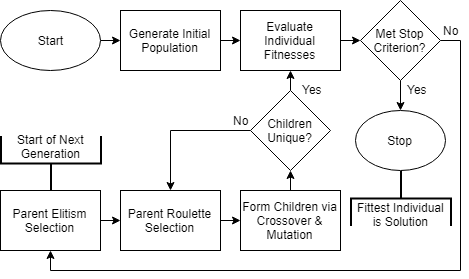
\includegraphics[width=1\linewidth]{Genetic_Algorithm_Basic}
\caption[Genetic Algorithm Block Diagram]{\small Block diagram of the GA approach.  This is for a typical genetic algorithm utilizing elitism and enforcing generational uniqueness.}
\label{fig:ga_block}
\end{figure}

\subsection{The GA Chromosome} \label{subsec:ga_chromosome}

Let $\mathcal{G} \defeq \left\{ 1,\, 2,\, \ldots,\, G \right\}$ be the set of generations used in the genetic algorithm and $\mathcal{I}_g \defeq \left\{ 1,\, 2,\, \ldots,\, I \right\},\, g \in \mathcal{G}$ be the set of individuals within generation $g$.  Each individual $i \in \mathcal{I}_g$ has a binary chromosome $\textbf{z}^{\left\{ ig \right\}}$ of length $S$.  $z_s^{\left\{ ig \right\}},\, s \in \mathcal{S}$, denoting each individual bit, or gene, of the chromosome, is defined as

\ifisdoublespacing
\begin{singlespacing}
\begin{equation}
z_s^{\left\{ ig \right\}} \defeq
	\begin{cases}
		1,& \text{if BS $s$ is selected by the VNB for individual $i$ in generation $g$;}\\
		\\
		0,& \text{otherwise.}
	\end{cases}
\end{equation}
\end{singlespacing}
\else
\begin{equation}
z_s^{\left\{ ig \right\}} \defeq
	\begin{cases}
		1,& \text{if BS $s$ is selected by the VNB for individual $i$ in generation $g$;}\\
		0,& \text{otherwise.}
	\end{cases}
\end{equation}
\fi

\subsubsection{Chromosome Fitness}

To evaluate the fitness of each chromosome in the GA approach, I assume that all demand over $\mathcal{R}$ is allocated to the closest resource relative to that resource's coverage radius.  That is, the demand allocated to a BS $s \in \mathcal{S}$ is all the demand located in the region $V_s$ such that

\begin{equation}
V_s = \left\{ p \in \mathcal{R} \mid \frac{d \left( p,\, s \right)}{b_s} \leq \frac{d \left( p,\, t \right)}{b_t} \; \forall s \neq t \right\}
\end{equation}

\noindent where $d \left( p,\, s \right)$ is the euclidean distance between an arbitrary point $p$ and BS $s$.  Let $\mathcal{S}' \subseteq \mathcal{S}$ be the set of resources that have been selected by an arbitrary chromosome (i.e., $z_s^{\left\{ ig \right\}} = 1,\, \forall s \in \mathcal{S}'$ and $z_s^{\left\{ ig \right\}} = 0,\, \forall s \not\in \mathcal{S}'$ for an arbitrary chromosome $\left\{ ig \right\}$).  By making this assumption, $\mathcal{S}'$ partitions $\mathcal{R}$ into a multiplicatively weighted Voronoi tessellation~\cite{Dobrin_areview,AURENHAMMER1984251} using the point locations of the selected BSs as the defining sites and BS coverage radii, $b_s,\, s \in \mathcal{S}'$, as weights; if all BSs in $\mathcal{S}'$ have homogeneous coverage radii (i.e., $b_s = b,\, \forall s \in \mathcal{S}'$), this partition is a standard unweighted Voronoi tessellation.

The region within the coverage radius of BS $s$ is denoted by $B_s$.  It is desired that $V_s$ be wholly contained within $B_s$ (i.e., $V_s \subseteq B_s$), but this is not guaranteed by the Voronoi tessellation assumption.  If $V_s$ is not wholly contained within $B_s$, BS $s$ is considered to be \emph{overcoverage}.  The total demand allocated to a selected resource $s \in \mathcal{S}'$ is $\sum_{n \in \mathcal{N}} \iint_{V_s} \lambda_n \left( x,\, y \right) \,dx \,dy$.  If the total demand allocated to BS $s$ exceeds $B_s$, BS $s$ is considered to be \emph{overcapacity}.

The fitness heuristic of each individual chromosome, $z^{\{ig\}}$, is assessed as the reciprocal of the chromosome's cost

\begin{equation} \label{eq:GAFit}
\mathrm{fitness}\left( z^{\left\{ ig \right\}} \right) = \frac{1}{\mathrm{cost}\left( z^{\left\{ ig \right\}} \right)}
\end{equation}

The cost of a given chromosome is the sum of the direct costs of the individual selected BSs and their associated overcoverage ($c_{\text{cov}}$) and overcapacity ($c_{\text{cap}}$) costs

\begin{multline} \label{eq:GACost}
\mathrm{cost}\left( \textbf{z}^{\left\{ ig \right\}} \right) = \sum_{s \in \mathcal{S}} \Biggl( c_s \; z_s^{\left\{ ig \right\}} + c_\text{cov} \; \ind{V_s \not\subseteq B_s} + \\ \left( c_\text{cap}^g - 1 \right) \; \max\left( 0,\, \sum_{n \in \mathcal{N}} \left( \iint_{V_s} \lambda_n\left( x,\, y \right)\, dx\, dy \right) - r_s \right) \Biggr)
\end{multline}

\noindent where $\ind{*}$ is the indicator function (\cref{eq:indicator}).

Resources that are overcoverage are not desired; solutions that assume some demand is unallocatable by being out of range should be consider less-than-feasible or completely infeasible from the outset.  In contrast, the overcapacity cost starts at zero and grows exponentially with each successive generation.  For early generations, this allows for inefficient or infeasible solutions to temporarily exist to seed later generations and improve generational diversity.  This increases the probability that the final solution (a local maxima) is the global maximum or closer to the global maximum of the fitness function.

It should be explicitly noted that the fitness (cost) of a given genome is monotonically non-increasing (non-decreasing) over $g \in \mathcal{G}$; a genome's fitness is constant over $g$ if the genome is not overcapacity, and strictly decreases every generation if the genome is overcapacity.

\subsection{Forming the Next Generation} \label{subsec:ga_next}

Once the fitness calculation of all of the individuals of the current generation has been performed, the next generation begins to form.

\subsubsection{Elitism and Selection}

Generating the next generation begins with selection.  First, I use elitism selection.  Under elitism selection, a defined number of the fittest individuals from each generation is selected as that generation's elitist members.  These elitist members, the $n$ fittest individuals of the generation, are cloned into the next generation without undergoing the genetic operators of crossover or mutation.  Through elitism, I ensure that the fittest individual of a given generation is not less fit than the previous generation's fittest individual.  The only exception comes from if the fittest individual's fitness decreases from inefficiency cost, but these are eventually removed as the overcapcity cost increases.

After elitism, standard selection occurs using roulette-wheel selection.  In roulette-wheel selection, the fitness of each individual to normalized to the total fitness of the generation and organized into a list.  From this list, a new list of the cumulative fitnesses is generated such that the cumulative fitness of individual $i$ is $\sum_{j = 1}^i \text{fitness} \left( z^{\left\{ jg \right\}} \right)$; the cumulative fitness of individual $I$ (i.e., the last individual in the generation) is thereby 1.  A random number, $P \sim \mathcal{U} \left( 0,\, 1 \right)$, is then generated.  The selected individual (or parent) is the first individual in the list that has a cumulative fitness value larger than $P$.

Under roulette-wheel selection, parents are each randomly selected with a probability given by

\begin{equation}
\text{P}\left( \text{individual $i$ of gen. $g$ is selected for gen. $g+1$} \right) = \frac{\text{fitness}\left( z^{\left\{ ig \right\}} \right)}{\sum_{i \in \mathcal{I}} \text{fitness}\left( z^{\left\{ ig \right\}} \right)}
\end{equation}

\subsubsection{Crossover}

Once selection has occurred, the individuals selected via roulette-wheel selection are paired off.  With a probability of $p_{\text{xov}}$, the pair undergoes crossover to form their two children which go on to the next generation; otherwise, the parents are cloned as their own children.  During crossover, the chromosomes of each pair of parents are mixed.  Typical forms of crossover include single-point, k-point, and uniform crossover, though there are other more exotic forms that are application specific.

I use uniform crossover as it has been suggested~\cite{Picek:2011:ECO:2184629.2184665} to be one of the best crossover operators in terms of general performance.  With uniform crossover, each gene in the chromosomes of the children are independently chosen from the parents' genomes with equal probability (i.e., 50\%).  A random binary mask of length $S$ is generated.  The first child inherits genes from the first parent where there is a $1$ in the mask and from the second parent where there is a $0$; the second child inherits the inverse.

Compared to single-point crossover, uniform crossover is also suggested to increase exploration of the search space as it severs the positional bias (linkage) of the bits in the genome~\cite{782011}; bits with possible spatial significance to one another no longer undergo crossover in segments like they would in single or k-point crossover.

\subsubsection{Mutation}

Once each child has been generated, each bit within the child's genome has an independent chance, $p_{\text{mut}}$, to mutate.  When a bit mutates, the bit flips from 1 to 0, or from 0 to 1.  Typically, the chance of each bit to mutate is $p_{\text{mut}} = \frac{1}{l}$, where $l$ is the length of the chromosome, which provides an average of one bit mutation per child~\cite{GREENWELL19951,Deb2011}.  For $\textbf{z}^{\left\{ ig \right\}}$, $p_{\text{mut}} = \frac{1}{S}$.

\subsubsection{Uniqueness}

In a traditional genetic algorithm, once mutation has been completed, the next generation of children has been completely generated.  However, it is possible for several children to be identical, reducing the overall genetic diversity of the generation and decreasing the algorithm's exploration of the search space.  To counter this possibility I enforce the ``uniqueness condition'', which is the assurance that each generation must be comprised of unique individuals.  If there are any individuals that are identical to others in the generation, all but one of the identical individuals are discarded from the generation.  The vacancies are then filled by a new set of generated children

\subsection{Stopping the GA} \label{subsec:ga_stop}

The GA iterates for a specified maximum number of generations $G$.  However, once the GA converges to a stable solution, it is worthwhile to halt the GA early to conserve time.  There are two halting conditions that control this.  First, the \emph{fitness halt} condition halts the GA if the fitness of the fittest individual remains unchanged for a number of sequential generations, $G_{\text{fit}}$.  Due to the fitness function's monotonicity, a solution under this condition is not overcapacity.  This halting condition is expected to provide a solution that is feasible to provide nearly 100\% demand satisfaction; a solution provided under fitness halt can be overcoverage, but being overcoverage should be unlikely if $c_{\text{cov}}$ is sufficiently high and if $\mathcal{S}$ is not too sparse to satisfy $\mathcal{R}$.

The second halting condition is the \emph{genome halt}.  Under this condition, the GA halts early if the genome of the fittest individual remains unchanged for a number of sequential generations, $G_{\text{gen}} \geq G_{\text{fit}}$.  Due to the fitness function's monotonicity, a solution under this condition is overcapacity; unlike the fitness halt condition, this allows for an infeasible (i.e., overcapacity) solution to evolve, especially when no solution is feasible.  The genome halt primarily contrasts with the fitness halt by forcing more generations to occur.  This allows for enough generations to pass so the overcapacity cost increases sufficiently that a hypothetical more feasible (i.e., less overcapacity) solution becomes more fit than the less feasible solution, and for enough generations to pass that it is statistically probable that the more feasible solution evolves.  Otherwise, an individual that satisfies the fitness halt condition also satisfies the genome halt condition; the fitness halt condition is a more strict form of convergence.

For both of these halting conditions, a minimum number of generations, $G_{\min} < G$, must first pass.  Once any halting condition occurs, the fittest individual of the final processed generation is the solution, with $\textbf{z}^{\left\{ ig \right\}}$ of the solution determining $z_s,\, s \in \mathcal{S}$.

In each case, the chromosome of the fittest individual when the GA halts is an approximate solution for the VNB's resource selection, $z_s$.  As the GA only handles the resource selection, it only represents a solution of the first stage (\cref{eq:SOPS1O,eq:SOPS1C1}) of the original stochastic optimization program (\cref{eq:SOPS1O,eq:SOPS1C1,eq:SOPS2O,eq:SOPS2C1,eq:SOPS2C2,eq:SOPS2C3,eq:SOPS2C4}).  That is, while joint resource selection has occurred and the process was informed by the demand to be satisfied (i.e., $\lambda_n$), the selected resources still need to be sliced to determine the allocations of those resources to specific VWNs.  This process of solving the second stage of the original optimization program can be adaptively handled to a hypothetical or real set of demand points using the adaptive slicing model (\cref{eq:ASMO,eq:ASMC1,eq:ASMC2,eq:ASMC3}) of \Cref{subsec:dep_slicing}.

The process of applying the GA approach is similar to the process used to apply the DEP approach of \Cref{sec:dep}.  An SP coordinates with a VNB, communicates its demands in the form of a demand intensity function, $\lambda \left( x,\, y \right)$, and the VNB concatenates the new demand into $\mathcal{N}$.  Then, the GA processes over $\lambda_n,\, n \in \mathcal{N}$ until either halting condition occurs or the maximum number of generations is reached.  The solution provided by the GA indicates the VNB's joint resource selection.  Finally, for any observed realization of demand points, the adaptive slicing model (\cref{eq:ASMO,eq:ASMC1,eq:ASMC2,eq:ASMC3}) is solved with that fixed resource selection, handling VWN construction in the short term.  The GA is rerun later as $\lambda_n$ changes for long term VWN construction.
\fi

\iftrue
\pagebreak
\chapter{Simulations and Results} \label{ch:sim}

In this chapter I evaluate the effectiveness of the sDEP (\Cref{sec:dep}) and GA (\Cref{sec:ga}) approaches as approximations of the two-stage stochastic optimization program presented in \Cref{sec:stochopt}.  I set up these approaches as a series of simulations and compare the costs, demand satisfaction, computation time, and general trends.  \improvement{Consider the reasoning for including these results.\\\emph{Why} are they included in this thesis?}First I present a set of preliminary results to evaluate the appropriateness of the simulations.  Then I present two cases that more closely represent the needs of an urban cellular network SP and the available resources to satisfy those needs; one case considers RPs with homogeneous resources while the other case considers RPs with heterogeneous resources.

\subsubsection{General Setup}

Unless stated otherwise, simulations are set up with the following assumptions.  BS locations are determined as a stationary PPP with a fixed number of BSs.  Demand point locations are generated independently for each SP $n \in \mathcal{N}$ in each scenario as a non-stationary PPP using $\lambda_n\left( x,\, y \right),\, x \in \left[ 0,\, X \right],\, y \in \left[ 0,\, Y \right]$, as the spatial intensity function, as described in \Cref{sec:networkdefs} (\cref{eq:nsPPPaccrej}).  Demand points have homogeneous demand (\cref{eq:demandintegral,eq:pointdemand}).  To compute $u_{ms}^{\left( \omega \right)}$, it is assumed that there is perfect propagation between demand points and BSs within the BSs' coverage radii (\cref{eq:umns_simp}).  To compute the fitness function for the GA approach (\cref{eq:GAFit,eq:GACost}), $\lambda_n$ is discretized into a grid of equal-sized square pixels with a given side length for the problem.  The demand of a given pixel is the product of $\lambda_n$ at the center of the pixel and the area of the pixel.  The demand allocated to a selected resource $s \in \mathcal{S}' \subseteq \mathcal{S}$ is the sum of the demand of all pixels within $V_s$, the resource's Voronoi cell.

Simulations were run on an Intel Core i7-4790K 4.00 GHz 4 real/8 virtual core CPU with 16 GB of DDR3 RAM.  I used CPLEX~\cite{Cplex} to solve the sDEP model (\cref{eq:sDEPO,eq:sDEPC1,eq:sDEPC2,eq:sDEPC3,eq:sDEPC4}) and the adaptive slicing model (\cref{eq:ASMO,eq:ASMC1,eq:ASMC2,eq:ASMC3}).  I used MATLAB to implement the GA and to generate the simulated region.  D uring the simulations, extraneous processes were culled to allow maximal use of computer resources.  For a given comparison to the sDEP, the GA results are provided from 50 independent runs using an identical data set except for the set of initial individuals.  The sDEP approach was solved across multiple values of $\alpha$.

\section{Preliminary Simulations} \label{sec:prelim}

This first considered problem is an initial simulation testing the performance of the sDEP and GA approaches for a general problem intended to be solved in less than 15 minutes.  This test was intended to show that the two approaches work correctly and present preliminary results later test cases.  \change{Only include if submitted}These results were compiled and collated in a paper submitted to the International Conference on Computing, Networking and Communications (ICNC 2019)~\cite{KTeague:BSSelection}\change{Double check}.

\subsection{Setup} \label{subsec:prelim_setup}

\begin{table}[ht]
\centering
\caption{Numerical Values of\\Relevant Parameters for Preliminary Simulations}
\begin{tabular}{|c|c|} 
\hline
Width, Height of Geographic Area ($X$) & 2 km x 2 km \\
\hline
Number of BSs ($S$) & 60 \\ 
\hline 
Number of Demand Points ($M$) & 75 \\ 
\hline 
Number of SPs ($N$) & 1 \\
\hline
Number of Sampled Scenarios ($O$) & $\{5,\, 10,\, \ldots,\, 50\}$ \iffalse 25 \fi \\ 
\hline 
BS cost ($c_s,\, \forall s \in \mathcal{S}$) & 1 \\ 
\hline 
BS capacity ($r_s,\, \forall s \in \mathcal{S})$ & 1.50 Mbps \\ 
\hline
BS range ($b_s,\, \forall s \in \mathcal{S}$) & 500 m \\
\hline 
Point Traffic Demand ($d$) & 0.178 Mbps \\ 
%\hline 
%Two-Stage Model Weight ($\alpha$) & 20\iffalse $\{5,\, 10,\, \ldots,\, 100\}$ \fi \\ 
\hline 
\hline
SSLT Approximation Depth ($L$) & 50 \\ 
\hline
SSLT Maximum Angular Frequency ($\omega_{\max}$) & $\frac{2 \; \pi}{30}$ \\
\hline 
SSLT Location Parameter ($\sigma$) & 0 \\ 
\hline 
SSLT Scale Parameter ($\mu$) & 1 \\ 
\hline
Pixel Grid Size & 100 x 100, 20 m \\
\hline 
\hline
Maximum Number of Generations ($G$) & 3000 \\ 
\hline
Minimum Number of Generations ($G_{\min}$) & 300 \\
\hline
Unchanged Generations Before Fitness Halt ($G_{\text{fit}}$) & 150 \\
\hline 
Unchanged Generations Before Genome Halt ($G_{\text{gen}}$) & 400 \\
\hline 
Number of Individuals per Generation ($I$) & 80 \\ 
\hline
Number of Elite Individuals per Generation & 4 \\
\hline 
Probability of Crossover ($p_\text{xov}$) & 0.7 \\ 
\hline
Probability of Mutation per bit ($p_\text{mut}$) & $\frac{1}{S} = 0.0167$ \\
\hline 
Overcoverage Cost ($c_\text{cov}$) & 3 \\
\hline
Overcapacity Cost ($c_\text{cap}$) & 1.015 \\
\hline
\end{tabular}
\label{tab:prelim_simval}
\end{table}

For these preliminary simulations, I use the parameter values shown in \Cref{tab:prelim_simval}.  There is only one SP, and its demand intensity function, $\lambda$, is generated using default location and scale parameters from the SSLT model ($\sigma = 0,\, \mu = 1$).  $\lambda$ is pixelated into a 100 by 100 grid of square pixels with 20 m side length, so that $\mathcal{R}$ is a region 2 km by 2 km.  The listed maximum angular frequency, $\omega_{\max}$, is in terms where each pixel is one unit (i.e., it correlates to a region that is 100 m by 100 m); in terms of absolute distance, $\omega_{\max}$ is scaled according to the side length (i.e., $\omega_{\max} = \frac{\pi}{300}$).  Resources are homogeneous and constructed to saturate the region's demands.

\subsection{Results} \label{subsec:prelim_results}

\section{Case I: Single SP with Homogeneous Resources} \label{sec:caseI}

\subsection{Setup} \label{subsec:caseI_setup}

\subsection{Results} \label{subsec:caseI_results}

\section{Case II: Single SP with Heterogeneous Resources} \label{caseII}

\subsection{Setup} \label{subsec:caseII_setup}

\subsection{Results} \label{subsec:caseII_results}

\iffalse


In Fig. \ref{fig:AlgSpeedupRunTime} is a comparison of the approach run times.  It shows the run times of both the DEP and genetic algorithm in terms of the speedup ratio and in absolute number of seconds.  As the number of scenarios sampled increases, the CPU run time of the sampled DEP increases exponentionally, and fails to converge to a final solution with 50 scenarios within the time limit of 15 minutes.  Except for the 5 scenario case, the genetic algorithm converges to a solution in less CPU time (125.8 seconds) than the sampled DEP.  When 20 scenarios are sampled, the DEP takes approximately 440\% of the time as the genetic algorithm; at 45 scenarios, this has increased to 4,630\%.  CPLEX is capable of parallelizing across the 8 CPU cores, allowing for the wall clock run time to be, at minimum, one-eighth the CPU run time.  In terms of the adjusted approximate ``wall clock" time, the genetic algorithm converges in less wall clock time than the sampled DEP for 25 or more sampled scenarios.

The trade off for the genetic algorithm's improved run time is that the solution provided is less optimal than the sampled DEP, as indicated by an increased cost for the VNB to build the VWN.  Fig. \ref{fig:VWNCompCost} compares the increasing cost of the sampled DEP as $\alpha$ increases with the cost of the various genetic algorithm solutions.  On average, the genetic algorithm incurs a 36\% increased cost in selecting the BSs for the VWN.  At minimum, the incurred cost is only 20\% than the sampled DEP, which implies the genetic algorithm might be terminating early, and a tighter solution might be found by increasing $G_\text{halt}$.  It should also be noted that one unit of cost is one additional BS being selected for the VWN, and the sampled DEP selections for $\alpha \geq 30$ have a cost of only 10 BSs.  Any variance that incurs one additional BS for the genetic algorithm incurs 10\% increased cost.  Increasing the number of BSs required to comprise the VWN would introduce additional granularity in $\mathcal{S}$ that might decrease the inefficiency of the genetic algorithm.  This was not done as this data set was chosen specifically so the sampled DEP would terminate within 15 minutes (i.e., in a reasonable amount of time); increasing the number of BSs available to the VNB drastically increases the time it would take the sampled DEP to converge to a solution.

There is a direct correlation between the number of BSs in the VWN and its capability for satisfying demand.  As the cost - and, therefore, the number of BSs - increases for a given solution, the average demand satisfaction trends towards 100\%, as shown in Fig. \ref{fig:VWNCompSatis}.  Because of this overallocation of resources, the genetic algorithm solutions have a very high demand satisfaction, averaging 99.9\% satisfaction and reaching 100\% for some solutions.  The worst performing genetic algorithm solution exceeded 99.1\% demand satisfaction.  The most expensive 10-BS sampled DEP solutions reach 99.2\% when slicing to the same set of demand point scenarios, $\Omega$, that determined the sampled DEP BS selection.

When the set of demand points change to a scenario no longer in $\Omega$, the sampled DEP performs very similarly.  Fig. \ref{fig:VWNCompSatisEval} shows the demand satisfaction for both the sampled DEP and genetic algorithm BS selections when sliced to a new set of scenarios as evaluated with Problem 3.  Here, the number of demand points increases to 200 points per scenario, each with 66.8 kbps rate demand, across 50 independent scenarios.  The demand satisfaction trend of the sampled DEP BS selection follows very closely to the original set of scenarios but hits a maximum of 99.0\% demand satisfaction with 10 BSs.  In comparison, the SP demand point scenarios are far more beneficial to the genetic algorithm, which reaches greater than 99.99\% demand satisfaction for all generated VWNs.  This is expected as a side effect of the increased number of points and scenarios more accurately describing a sampling of the original SSLT demand density field of the SP, $\rho$.

\improvement{Start this chapter ASAP.  Start running Case I data now.}

\textit{In this chapter I will be introducing four different cases to test the provided approximation approaches.  The first will be the test case used in my conference paper (one SP, with homogeneous resources).  The second will be an expansion of the test case used in my conference paper, but with heterogeneous resources.  The third will extend to service multiple similar cellular SPs.  The fourth will extend to a case with multiple SPs with various, specialized demands.}

\section{VWN Construction for a Single SP} \label{sec:onesp}

\textit{Lead into the first two cases, which test the approaches while using a single SP.}

\subsection{Case I: Homogeneous Urban Cellular Network} \label{subsec:onesp_homres}

\improvement{Start this!}

\textit{Basically as presented in my conference paper.  One SP, homogeneous resources within the RPs.  Might need to use a new data set, though, with a larger data set.}

\subsection{Case II: Impact of Heterogeneous Resources} \label{subsec:onesp_hetres}

\textit{Same as Case I, but with heterogeneous resources within the RPs.  Need to understand how this changes the approaches.}

\section{VWN Construction for Multiple SPs} \label{sec:mulsp}

\textit{Lead into the second two cases (should I have more?), which test using multiple SPs to satisfy from the same set of resources.}

\subsection{Case III: Two Similar Urban Cellular Networks} \label{subsec:mulsp_sim}

\textit{First consider a case with two SPs with similar demands.  Overlapping cellular networks.  Could see how the approaches behave while two SPs partially overlap.}

\subsubsection{Homogeneous Resources} \label{subsubsec:mulsp_sim_homres}

\textit{If it appears that the difference between Case I and Case II (sections \ref{subsec:onesp_homres} and \ref{subsec:onesp_hetres}) is worth further consideration, then analyze here with homogeneous resources.  Otherwise, a single comparison should be sufficient.}

\subsubsection{Heterogeneous Resources} \label{subsubsec:mulsp_sim_hetres}

\textit{As for the previous subsubsection (\ref{subsubsec:mulsp_sim_homres}), but consider with heterogeneous resources.}

\subsection{Case IV: SPs with Specialized Demands} \label{subsec:mulsp_spec}

\textit{This is the major case that is the extension of my work.  Case I (\ref{subsec:onesp_homres}) analyzed what happens with a single SP, Case II (\ref{subsec:onesp_hetres}) expanded that to heterogeneous resources, and Case III (\ref{subsec:mulsp_sim}) added an additional similar SP, but Case IV considers when there are several SPs and with their own considerations and unique demands.  Need to consider what these SPs look like.  One would be a cellular network like in Case I (moderate to high number of users, moderate demand).  Another could be a streaming service (few users, high individual demand).  Another an emergency service (very low number of users and demand, but requiring virtually 100\% demand satisfaction - see note below).  What other SPs should I consider?}

\textit{\textbf{Note}: I need to consider how to accurately label demand satisfaction within the approaches.  In effect, this would be controlled by $\alpha$ for the (sampled) DEP and controlled by $\beta$ or some such for the genetic algorithm.  I should investigate this at some point of the thesis, probably within their appropriate sections in chapter \ref{ch:approaches} (DEP: \ref{sec:dep} and GA: \ref{sec:ga}).}

\subsubsection{Homogeneous Resources} \label{subsubsec:mulsp_spec_homres}

\textit{As for Case III (\ref{subsec:mulsp_sim}), if a considerable difference was detected between Cases I and II (\ref{subsec:onesp_homres} and \ref{subsec:onesp_hetres}), consider analyzing the case with homogeneous resources and}

\subsubsection{Heterogeneous Resources} \label{subsubsec:mulsp_spec_hetres}

\textit{also with heterogeneous resources.}
\fi

\fi

\iftrue
\pagebreak
\chapter{Conclusions} \label{ch:conc}

\change{Old work\\Update and Remove!}%
\textit{Consider conclusions of my work.  I don't think this chapter would be long, but condense my findings into some coherent thoughts, and redirect to what they are.  Also expound on some of the further work that my research could be expanded to (e.g., further use cases investigating my approaches, use of (meta)heuristics other than a genetic algorithm to approximate the optimization problem, improve the basic capacity function used in my optimization model).}

\section{Considerations for Future Work} \label{sec:futurework}

\info{Filled as ideas come to mind during writing}

\noindent -- Other traffic demand models (log-normal mixtures, $\alpha$-stable)\info{See note.\\Integrate.}\footnote{In general, network traffic and the resource deployments that they are meant to model tend to exhibit characteristics of heavy-tailed spatial distributions.  It has been shown that traffic distributions in cellular networks can be more accurately approximated as a mixture of log-normal distributions~\cite{5936263, 6757900}; Lee et al.~\cite{6757900} describe that nonmixtures capture the distribution for a single moment while mixtures capture the distribution as it changes with time and place.  Similarly, Zhou et al.~\cite{7202841} have shown that distributions of deployed BSs can be accurately approximated as a $\alpha$-stable distribution.  The latter case might be explained through the central limit theorem, as the sum of power-law distributed (Paretian tailed) random variables, such as those describing traffic in telephone networks~\cite{PhysRevE.72.026116}, will tend towards an $\alpha$-stable distribution.  I use neither in this thesis as $\alpha$-stable distributions do not generally have a closed-form probability density function (PDF), rendering use non-trivial, and log-normal mixtures require tuning multiple parameters, adding additional complexity.}\\%
% Moved the footnote from \Cref{ch:networkdefs}, where it created an overly long footnote while providing no real new information.  These sorts of details could be properly integrated here into the conclusion.  Move out of footnote and place in mainbody text.
-- Rate normalization that varies with distance (i.e., non-binary $\tilde{u}_{ms}$)\\%
-- Other heuristic approaches (e.g., particle swarm optimization, simulated annealing, deep learning approaches)\\%
-- \info{$\beta$ already works this way for the GA implementation, as it applies a constant to $\lambda\left( x,\, y \right)$.} Altering $\alpha$ to vary according to the demand points of the various SPs, allowing for each SP to independently control the desired demand satisfaction of their network.\\%
-- Handling varying values of $b_s$ within the GA\\%
-- Improve the GA implementation such that it uses some form of integration of $\lambda\left( x,\, y \right)$\\%
-- Adjust the demand of each demand point to be based on the expected number of demand points, not the exact amount of demand in the region; allow for different numbers of demand points than a fixed value so that it accurately reflects a PPP.
\fi

\iffalse
\pagebreak
\chapter{Derivations} \label{ch:derive}

\begin{align}
\text{Area} &= \int_X \int_Y \rho\left( x,\, y \right) dy \, dx \\
&= \int_X \int_Y \exp\left( \sigma \; \rho^S \left( x,\, y \right) + \mu \right) dy \, dx \\
&= \int_X \int_Y \exp\left( \frac{\sigma}{\sigma^G} \; \left( \rho^G\left( x,\, y \right) - \mu^G \right) + \mu \right) dy \, dx \\
&= \int_X \int_Y \exp\left( \frac{\sigma}{\sigma^G} \; \rho^G\left( x,\, y \right) - \frac{\sigma}{\sigma^G} \; \mu^G + \mu \right) dy \, dx \\
&= \int_X \int_Y \exp\left( \hat{\sigma} \; \rho^G\left( x,\, y \right) + \hat{\mu} \right) dy \, dx \\
& \hspace{1in} \text{where $\hat{\sigma} = \frac{\sigma}{\sigma^G}$ and $\hat{\mu} = \mu - \frac{\sigma}{\sigma^G} \; \mu^G$} \nonumber \\
&= \int_X \int_Y \exp\left( \hat{\sigma} \frac{1}{L} \sum_{l = 1}^L \cos\left( i_l x + \phi_l \right) \; \cos\left( j_l y + \psi_l \right) + \hat{\mu} \right) dy \, dx \\
& \hspace{1in} \text{where $i_l,\, j_l \sim \mathcal{U}\left( 0,\, 2\pi \right)$ and $\phi_l,\, \psi_l \sim \mathcal{U}\left( 0,\, \omega_{\max} \right)$} \nonumber \\
&= e^{\hat{\mu}} \int_X \int_Y \exp\left( \frac{\hat{\sigma}}{L} \sum_{l=1}^L \cos\left( i_l x + \phi_l \right) \; \cos\left( j_l y + \psi_l \right) \right) dy \, dx \\
&= e^{\hat{\mu}} \int_X \int_{U=Y} \exp\left( u \right) \frac{-L}{\hat{\sigma} \sum_{l=1}^L j_l \; \cos\left( i_l x + \phi_l \right) \; \sin\left( j_l y + \psi_l \right)} du \, dx \\
& \hspace{1in} \text{where $u = \frac{\hat{\sigma}}{L} \sum_{l=1}^L \cos\left( i_l x + \phi_l \right) \; \cos\left( j_l y + \psi_l \right)$} \nonumber \\
& \hspace{1in} \text{and $du = \frac{-\hat{\sigma}}{L} \sum_{l=1}^L j_l \cos\left( i_l x + \phi_l \right) \; \sin\left( j_l y + \psi_l \right) dy$} \nonumber \\
& \hspace{1in} \text{or $dy = \frac{-L}{\hat{\sigma} \sum_{l=1}^L j_l \cos\left( i_l x + \phi_l \right) \; \sin\left( j_l y + \psi_l \right)} du$} \nonumber \\
&= \frac{-e^{\hat{\mu}} L}{\hat{\sigma}} \int_X \left. \exp\left( u \right) \right\rvert_{u = U \sim Y} \left. \frac{1}{\sum_{l=1}^L j_l \cos\left( i_l x + \phi_l \right) \; \sin\left( j_l y + \psi_l \right)} \right\rvert_{y = a_0 x + b_0}^{a_1 x + b_1} dx \\
&= \frac{-e^{\hat{\mu}} L}{\hat{\sigma}} \int_X \exp\left( \frac{\hat{\sigma}}{L} \sum_{l=1}^L \cos\left( i_l x + \phi_l \right) \; \cos\left( j_l y + \psi_l \right) \right) * \nonumber \\
& \hspace{1.9in} \frac{1}{\sum_{l=1}^L j_l \cos\left( i_l x + \phi_l \right) \; \sin\left( j_l y + \psi_l \right)} \Biggr\rvert_{y = a_0 x + b_0}^{a_1 x + b_1} dx \\
&= \frac{-e^{\hat{\mu}} L}{\hat{\sigma}} \int_X \Biggl[ \exp\left( \frac{\hat{\sigma}}{L} \sum_{l=1}^L \cos\left( i_l x + \phi_l \right) \; \cos\left( j_l \left( a_1 x + b_1 \right) + \psi_l \right) \right) * \nonumber \\
& \hspace{1.9in} \frac{1}{\sum_{l=1}^L j_l \cos\left( i_l x + \phi_l \right) \; \sin\left( j_l \left( a_1 x + b_1 \right) + \psi_l \right)} \Biggr] - \nonumber \\
& \hspace{0.9in} \Biggl[ \exp\left( \frac{\hat{\sigma}}{L} \sum_{l=1}^L \cos\left( i_l x + \phi_l \right) \; \cos\left( j_l \left( a_0 x + b_0 \right) + \psi_l \right) \right) * \nonumber \\
& \hspace{1.9in} \frac{1}{\sum_{l=1}^L j_l \cos\left( i_l x + \phi_l \right) \; \sin\left( j_l \left( a_0 x + b_0 \right) + \psi_l \right)} \Biggr] \\
&= \frac{-e^{\hat{\mu}} L}{\hat{\sigma}} \int_X \Biggl[ \exp\left( \frac{\hat{\sigma}}{L} \sum_{l=1}^L \cos\left( i_l x + \phi_l \right) \; \cos\left( j_l a_1 x + j_l b_1 + \psi_l \right) \right) * \nonumber \\
& \hspace{1.9in} \frac{1}{\sum_{l=1}^L j_l \cos\left( i_l x + \phi_l \right) \; \sin\left( j_l a_1 x + j_l b_1 + \psi_l \right)} \Biggr] - \nonumber \\
& \hspace{0.9in} \Biggl[ \exp\left( \frac{\hat{\sigma}}{L} \sum_{l=1}^L \cos\left( i_l x + \phi_l \right) \; \cos\left( j_l a_0 x + j_l b_0 + \psi_l \right) \right) * \nonumber \\
& \hspace{1.9in} \frac{1}{\sum_{l=1}^L j_l \cos\left( i_l x + \phi_l \right) \; \sin\left( j_l a_0 x + j_l b_0 + \psi_l \right)} \Biggr] \\
&\text{The next step is unfinished} \nonumber \\
&= \frac{-e^{\hat{\mu}} L}{\hat{\sigma}} \int_X \Biggl[ \exp\left( \frac{\hat{\sigma}}{2L} \sum_{l=1}^L \cos\left( \left( i_l - j_l a_1 \right) x + \phi_l - j_l b_1 - \psi_l \right) \; \cos\left( j_l a_1 x + j_l b_1 + \psi_l \right) \right) * \nonumber \\
& \hspace{1.9in} \frac{1}{\sum_{l=1}^L j_l \cos\left( i_l x + \phi_l \right) \; \sin\left( j_l a_1 x + j_l b_1 + \psi_l \right)} \Biggr] - \nonumber \\
& \hspace{0.9in} \Biggl[ \exp\left( \frac{\hat{\sigma}}{L} \sum_{l=1}^L \cos\left( i_l x + \phi_l \right) \; \cos\left( j_l a_0 x + j_l b_0 + \psi_l \right) \right) * \nonumber \\
& \hspace{1.9in} \frac{1}{\sum_{l=1}^L j_l \cos\left( i_l x + \phi_l \right) \; \sin\left( j_l a_0 x + j_l b_0 + \psi_l \right)} \Biggr] \\
\end{align}
I believe this integral to be unsolvable with primitive functions.  There may be a solution using the CDF of a Gaussian random variable, or the error function (erf), complementary error function (erfc), or Q function.

Now I will try to prove that altering the magnitude of $\lambda$ linearly changes the probability of the number of points in a given area in a PPP.

\begin{align}
P\left\{ N\left( B \right) = n \right\} &= \frac{\left( \lambda | B | \right)^n}{n!} \, e^{-\lambda | B |} \\
& \text{Doubling $\lambda$ should double the number of points in $| B |$} \nonumber \\
P\left\{ N\left( B \right) = 2n \right\} &= \frac{\left( 2 \lambda | B | \right)^{2n}}{\left( 2n \right)!} \, e^{-2 \lambda | B |} \\
&= \frac{\left( 2 \lambda | B | \right)^n \left( 2 \lambda | B | \right)^n}{\left( n \right)! \frac{\left( 2n \right)!}{\left( n \right)!}} e^{-\lambda | B |} e^{-\lambda | B |} \\
&\text{The next step is unfinished} \nonumber \\
&= \frac{2^n 2^n n!}{\left( 2n \right)!}
\end{align}

\fi

\bibliography{KT_Thesis}
\bibliographystyle{IEEEtran}

\end{document}